\documentclass{report}
\usepackage[T1]{fontenc}
\usepackage[utf8]{inputenc}
\usepackage[english]{babel}
\usepackage{url}
\usepackage[hidelinks]{hyperref}
\usepackage{graphicx}
\usepackage{booktabs}
\usepackage{caption}
\usepackage{tabularx}
\usepackage{multirow}
\usepackage{parallel}
\usepackage{pdfcolparallel}
\usepackage{multicol}
\usepackage{amsmath}
\usepackage{amsfonts}
\usepackage{amssymb}
\usepackage{xcolor}
\usepackage{rotating}
\author{Enrico Franco}
\title{Software Engineering - Morisio Maurizio \\
	Lectures notes}
\begin{document}
\maketitle
\tableofcontents

\chapter{Introduction}
Microsoft Windows is installed in 90\% of the machines, including all version still in use. Windows API is a very difficult one, because there are a lot of versions that are still used and therefore many functions are there to guarantee backward compatibility.

Windows operating systems have all features required for 64-bit architecture and multi-core systems. Essential features include:
\begin{itemize}
\item Physical and virtual memory;
\item File systems (I/O, files, directories);
\item Multi-tasking (concurrency) with processes and threads;
\item Communication and synchronization;
\item Security.
\end{itemize}
Windows does support many standards. C library is always available but you cannot fully exploit Windows with it. For example, it is not possible to lock a file or a part of it, mapping a file into main memory and organize inter-process communication.

\section{Programming principles}
Windows APIs are defined in C language, going beyond standard C therefore reducing code portability but increasing code functionality. They are different from other standard, they require their own coding style and technique and use threads, not processes, as a basic unit of execution.

Including \texttt{windows.h}, most of the required data are already included. Windows contains many functions to perform the same or similar operations, each one with numerous parameters and flags and occasional artifacts from 16-bit versions.

\paragraph{Windows names}
\begin{itemize}
\item Function names are long and descriptive;
\item Variables are long and descriptive, often use "Hungarian" notation.
\item Symbolic constants and flags explain their meaning.
\end{itemize}

Nearly every resource is a \emph{kernel object}. Objects are identified and referenced by handle. Handle objects are of type \texttt{HANDLE}, similar to UNIX file descriptor or process id. \texttt{HANDLE}s are gray boxes, hence they must be manipulated by Windows APIs and theyinclude files, pipes, processes, threads, etc.

Predefined and descriptive data types are expressed in upper case (\texttt{BOOL}, \texttt{DWORD}, etc.) avoiding the \texttt{*} operator and making name distinctions (\texttt{LPTSTR}, i.e.\@ Long Pointer To STRing defined as \texttt{TCHAR*}).

\paragraph{Coding systems}
Windows supports executable code built in 16 (Win16), 32 (Win32) and 64 (Win64) bits. 16-bit versions are only for backward compatibility, while 32-bit versions run on 64-bit architecture but cannot exploit the larger address space. Most of the difference concern the pointer size. 

Four different coding strategies are possible:
\begin{itemize}
\item 8-bit only;
\item Unicode only;
\item 8-bit and Unicode with generic code;
\item 8-bit and Unicode with run-time selection.
\end{itemize}
To assume maximum flexibility and source portability, define all characters and strings using generic type \texttt{TCHAR} and calculate lengths using \texttt{sizeof(TCHAR)}. In fact, \texttt{TCHAR} is automatically mapped on ANSI ASCII coding when it is on 8-bits or Unicode UTF-16 coding when it is mapped on 16-bits.

\subparagraph{Generic strings}
Constant strings are expressed in one of the three forms:
\begin{itemize}
\item \textbf{ANSI C}: \texttt{"8-bit characters"};
\item \textbf{ANSI C}: \texttt{L"16-bit characters"};
\item \textbf{A macro}: \texttt{\_T("Generic characters")}; The \texttt{TEXT} macro is the same as \texttt{\_T}.
\end{itemize}

To select coding system include \texttt{\#define UNICODE} to get \texttt{WCHAR} in all source modules, before including \texttt{<windows.h>}.
\begin{verbatim}
#ifdef UNICODE
  #define TCHAR WCHAR
#else
  #define TCHAR CHAR
#endif
\end{verbatim}
To make available a wide class of string processing and I/O functions include \texttt{\#define \_UNICODE} consistently with \texttt{UNICODE}. To get generic C library text macros and functions include \texttt{\#include <tchar.h>} after \texttt{<windows.h>} and use the \emph{generic C} library for all string functions.

\paragraph{Main program definition}
Pay attention on how the main header is defined. To ensure correct operations in all combination use \texttt{int \_tmain(int argc, LPTSTR argv[])}. This is expanded to \texttt{main} or \texttt{wmain} depending on definition of \texttt{\_UNICODE}.

Directive \texttt{\#define \_CRT\_SECURE\_NO\_WARNINGS} removes annoying warnings from project in Visual Studio.
\chapter{The software process}
The \emph{software process} is not new. It is just a matter of applying engineering approach to software production.

The main difference with respect to tradition engineering is that software engineering is only 50 years old and it has limited theories and laws. Those issues affect the maturity of customers and managers which, nowadays, is very variable.

\section{Activities}
Goal is to produce software, including documents, data and code, with defined, predictable process properties (cost, duration, \dots) and product properties which defines product quality (functionality, reliability, \dots).
\begin{enumerate}
\item Requirements: what the software should do;
\item Design: definition and organization of physical (files and directories) and logical (functions, classes, packages, subsystems) units;
\item Implementation: source code writing (and generation of executable code) and units integration.
\end{enumerate}
Logically, each activity depends on the previous one. Those dependencies make software not soft.

First approach is to do these activities in sequence. In practice, feedbacks and recycles must be provided. At the end of each activity, a document (or source code) is produced.

\paragraph{The V \& V activities}
The software process may have a lot of defects. The idea is to find and fix them as soon as they are discovered. \emph{Verification and validation} activities control the correctness of:
\begin{itemize}
\item the requirements: customer needs are known and understood and the requirements document is consistent;
\item the design: it is capable of supporting the requirements and it is consistent;
\item the code: it is capable of supporting the requirements and the design and it is consistent (syntactic checks).
\end{itemize}

\paragraph{The management activities}
\begin{itemize}
\item Project management
\begin{itemize}
\item Assigns work and monitors progress;
\item Estimates and control budget.
\end{itemize}
\item Configuration management
\begin{itemize}
\item Identifies and stores documents and units;
\item Keeps track of relationships and history (version control).
\end{itemize}
\item Quality assurance
\begin{itemize}
\item Defines quality goals;
\item Defines how work will be done;
\item Controls results;
\item May repeat some V \& V activities.
\end{itemize}
\end{itemize}

\begin{figure}[hbtp]
\centering
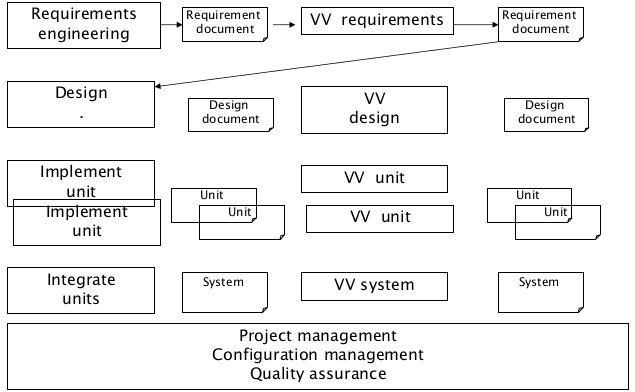
\includegraphics[scale=0.5]{images/software_activities.png}
\caption{Production + VV activities}
\end{figure}

\section{Phases}
Development is only the first part of the game. 

\begin{figure}[hbtp]
\centering
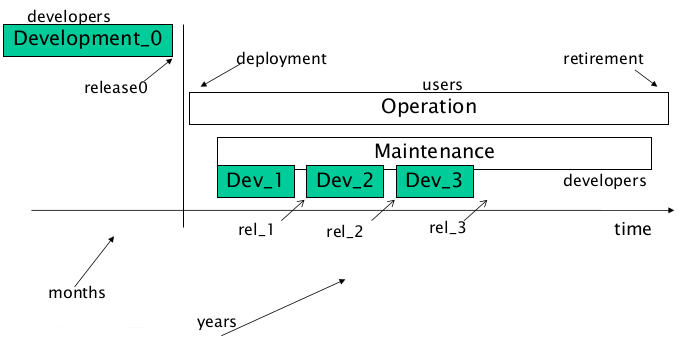
\includegraphics[scale=0.4]{images/software_phases.jpg}
\caption{Software phases}
\end{figure}

\paragraph{Operation}
\emph{Operation} is made by the users until retirement. Companies try to keep software as long as possible, i.e.\@ tens of years. A software used for a short amount of time, is not a good one. 

\paragraph{Maintenance}
\emph{Maintenance} can be seen as a sequence of developments. It starts immediately after the first release and lasts until retirement.

First development is usually longer, next developments are constrained by previous ones and related choices. After years, the constraints are so many that changes become impossible.

\begin{figure}[hbtp]
\centering
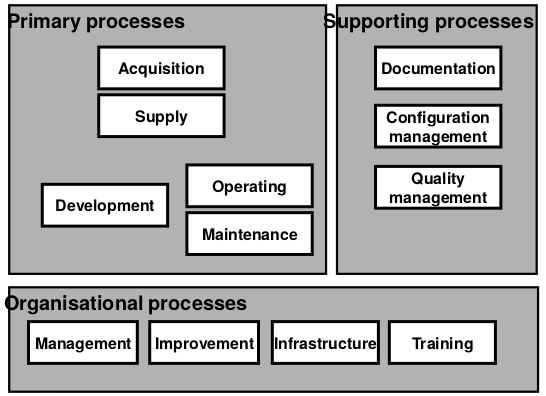
\includegraphics[scale=0.4]{images/iso_iec_12207.png}
\caption{ISO/IEC 12207}
\end{figure}

\section{The system process}
\emph{Embedded software} requires system process:

\begin{enumerate}
\item System requirements;
\item System design;
\item software development (requirements, design, implementation, test and integration);
\item System integration and test.
\end{enumerate}

\begin{figure}[hbtp]
\centering
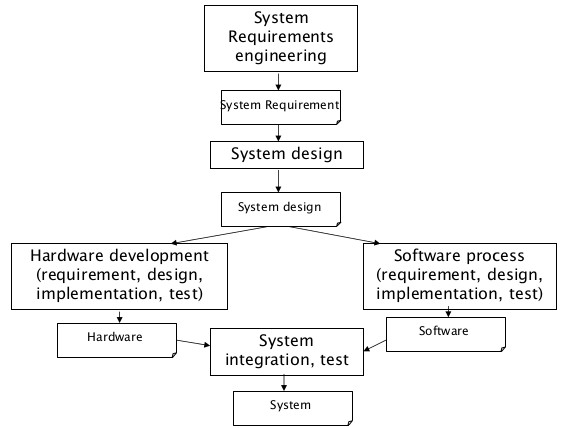
\includegraphics[scale=0.4]{images/system_process.jpg}
\caption{The system process}
\end{figure}
\chapter{Requirements engineering}
\emph{Requirements engineering} is about defining the product properties \emph{above starting development}. Without it, product properties may be unclear and testing phase is not feasible.

\textbf{Elicitation} consists of collecting information from the customer and producing an informal description, e.g.,\@ scratch or notes. This document is subjected to an analysis and formalization phase which produces the requirement document, a formal document which needs a final inspection in order to check its quality.

\begin{figure}[hbtp]
\centering
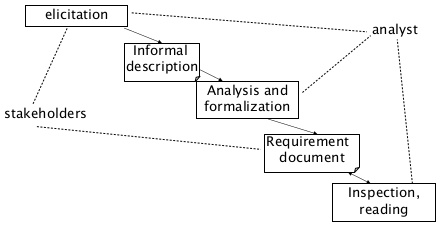
\includegraphics[scale=0.4]{images/re_phases.png}
\caption{Requirement engineering}
\end{figure}

A \textbf{requirement} is a description of a system or a service and its constraints. Requirements have different levels of abstraction and formality and they may be distinguished in functional and not functional.

Informal requirements often are not precisely stated. Ambiguous requirements may be interpreted in different ways by developers and users. In principle, requirements should be both complete and consistent.
\begin{itemize}
\item Complete: they should include descriptions of all facilities required;
\item Consistent: there should be no conflicts or contradictions in the descriptions of the system facilities.
\end{itemize}
In practice, it is impossible to produce a complete and consistent requirement document, also because there are no mathematical models or languages which can represent requirements.

\section{Defects}
\paragraph{Omission/Incompleteness}
Some information are not written. This defect is very difficult to find and fix.

\paragraph{Incorrect fact}
This defect is less difficult to find and fix. It may refer to a common knowledge.

\paragraph{Inconsistency/Ambiguity}
Some information are not strictly specified.

\paragraph{Extraneous information}
Overspecification: some information are not part of the requirement document.

\paragraph{Redundancy}
The same concept is repeated multiple times and possibly in slightly different ways, leading to ambiguity. Redundancy has to be avoided because, during the evolution of the document, it is possible to modify some concepts causing ambiguity.

\section{Techniques}
The requirement document is built using different techniques and it provides a \emph{structure}. The structure may change, order of parts is less important than precise description of parts.
\begin{enumerate}
\item Overall description;
\item Stakeholders;
\item Context diagram and interfaces;
\item Requirements
\begin{itemize}
\item Functional;
\item Non functional;
\item Domain;
\end{itemize}
\item Use case diagram;
\item Scenarios;
\item Glossary;
\item System design.
\end{enumerate}

\paragraph{Stakeholders}
A \emph{stakeholder} identifies a role or a person with an interest (stake) in the system to be built. Listing relevant stakeholders is essential to consider relevant points of view and therefore relevant requirements for the system.

\paragraph{Context diagram}
The \emph{context diagram} defines what is inside the system to be developed, what is outside and the interfaces between inside and outside. Outside entities interacting with the system are \textit{actors}. Stakeholders represent a subset of actors.

Context diagram and interfaces are essential to agree on what is the scope of the system.

\subparagraph{Interfaces}
Formal notations are an effective technique for interface specification.
Three types of interface may have to be defined:
\begin{itemize}
\item User interfaces, GUIs;
\item Procedural interfaces;
\item Data exchanged.
\end{itemize}

\paragraph{Numbering and type}
\begin{itemize}
\item Functional: general and informal description of services and behaviors provided by the system;
\item Non-functional: constraints on how functional requirements have to be implemented.
\end{itemize}

\subparagraph{Functional}
They can be inferred after the first reading of the informal description. Functional requirements are not all at the same level (i.e.,\@ complexity), in fact it is possible to introduce a hierarchy in requirements enumeration. Naming and numbering functional requirements is very useful because it helps their management (ready, released, paid) and their testing.

\subparagraph{Non-functional}
Non-functional requirements may be more critical than functional ones. If these are not met, the system is useless.
\begin{itemize}
\item Product requirements: requirements which specify that the delivered product must behave in a particular way (execution speed, reliability \dots);
\item Organizational requirements: requirements which are a consequence of organizational policies and procedures (process standard used, implementation requirements, \dots);
\item External requirements: requirements which arise from factors which are external to the system and its development process (interoperability requirements, legislative requirements, \dots).
\end{itemize}
Often, organizational and external requirements are taken for granted by the customer, therefore they are more difficult to extract.

ISO 9126 / ISO 25010 defines six properties of software systems associated to each function, not to the whole system.
\begin{itemize}
\item Functionality;
\item Reliability;
\item Usability\footnote{Waiting times < 0.1 sec are not perceived, while waiting > 1 sec are considered annoying.};
\item Efficiency;
\item Maintainability;
\item Portability.
\end{itemize}

Non-functional requirements must be \emph{measurable}, otherwise they are not testable, and therefore useless.

Conflicts between different non-functional requirements are common in complex systems. It is possible to rank the requirements in order to understand which are the most important.

\subparagraph{Domain requirements}
\emph{Domain requirements} are derived from the application domain and describe system characteristics and features reflecting the domain. They can be new functional requirements, constraints on existing requirements or define specific behaviors. If domain requirements are not satisfied, the system may be unworkable.

\textbf{Understandability}: requirements are expressed in the language of the application domain and they are often not understood by software engineers developing the system.

\textbf{Implicitness}: domain specialists understand them so well that they do not think of making the domain requirements explicit.

\paragraph{Glossary}
\emph{Glossary} is important to ``standardize'' terms. A class diagram can be used to refine glossary.

\paragraph{Scenarios}
A \emph{scenario} is a sequence of steps (events) that describe a typical interaction with the system. Each step should correspond to a function. In this way, it is possible to notice if a function is missing.

A scenario is also a \emph{test case}. Describing the interesting scenarios will help to perform 
coherent tests.

\paragraph{Use cases}
A \emph{use case} is a set of scenarios with common goal.

\paragraph{System design}
\emph{System design} identifies subsystems (software and not) composing the system.
\chapter{UML Class diagram}
How to identify important concepts on the environment:
\begin{enumerate}
\item Underline nouns: nouns are candidates for classes, attributes, \dots;
\item Define classes;
\item Define attributes for classes;
\item Underline verbs: verbs are candidates for relationships;
\item Define relationships;
\item Define multiplicities.
\end{enumerate}

\section{University}
Define a class diagram for a glossary for university. In a university there are different classrooms, offices and departments. A department has a name and it contains many offices. A person working at the university has a unique ID and can be a professor or an employee.

\begin{itemize}
\item A professor can be a full, associate or assistant professor and he/she is enrolled in one department.
\item Offices and classrooms have a number ID
\item A classroom has a number of seats.
\item Every Employee works in an office.
\item An employee enters and exits a classroom.
\end{itemize}

\subsection{Solution}
Define a class diagram for a glossary for \colorbox{yellow}{university}. In a university there are different \colorbox{yellow}{classrooms}, \colorbox{yellow}{offices} and \colorbox{yellow}{departments}. A department has a \colorbox{cyan}{name} and it \colorbox{green}{contains} many offices. A \colorbox{yellow}{person} \colorbox{green}{working} at the university has a unique \colorbox{cyan}{ID} and can be a \colorbox{yellow}{professor} or an \colorbox{yellow}{employee}.

\begin{itemize}
\item A professor can be a full, associate or assistant professor and he/she \colorbox{green}{is enrolled} in one department.
\item Offices and classrooms have a number \colorbox{cyan}{ID};
\item A classroom has a \colorbox{cyan}{number of seats}.
\item Every employee \colorbox{green}{works} in an office.
\item An employee \colorbox{green}{enters and exits} a classroom.
\end{itemize}

A possible strategy to represent different professor roles is to have a type field in the \emph{Professor} class or use a generalization-specialization pattern to identify the possible types. If there is no peculiar properties in the sub-classes, it is good practice to avoid the use of specialization. A ``discriminant'' attribute should be sufficient and it is preferable.

\begin{figure}[hbtp]
\centering
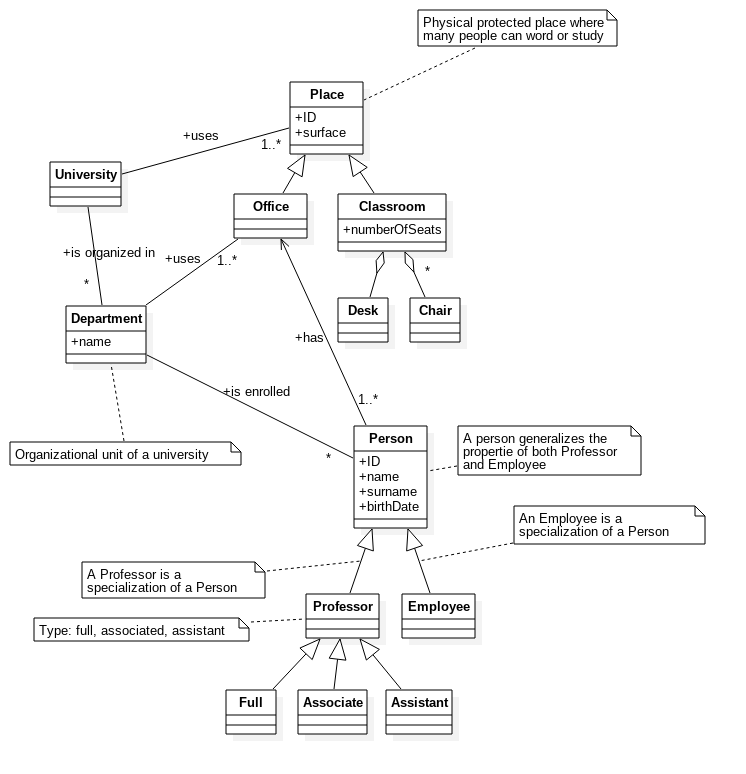
\includegraphics[scale=0.45]{exercises/classDiagram_university.png}
\caption{University - Class Diagram}
\end{figure}

\newpage
\section{Flights}
Draw a class diagram to define the glossary for management of flights and pilots.

An airline operates flights. Each airline has an ID. Each flight has an ID, a departure airport and an arrival airport: an airport has a unique identifier. Each flight has a pilot and a co-pilot, and it uses an aircraft of a certain type; a flight has also a departure time and an arrival time.

An airline owns a set of aircrafts of different types. An aircraft can be in a working state or it can be under repair, and in a particular moment an aircraft can be landed or airborne.

A company has a set of pilots: each pilot has an experience level: 1 is minimum, 3 is maximum.

A type of aircraft may need a particular number of pilots, with a different role (Ex. captain, co-pilot, navigator): there must be at least one captain and one co-pilot, and a captain must have a level 3.

\begin{sidewaysfigure}
\centering
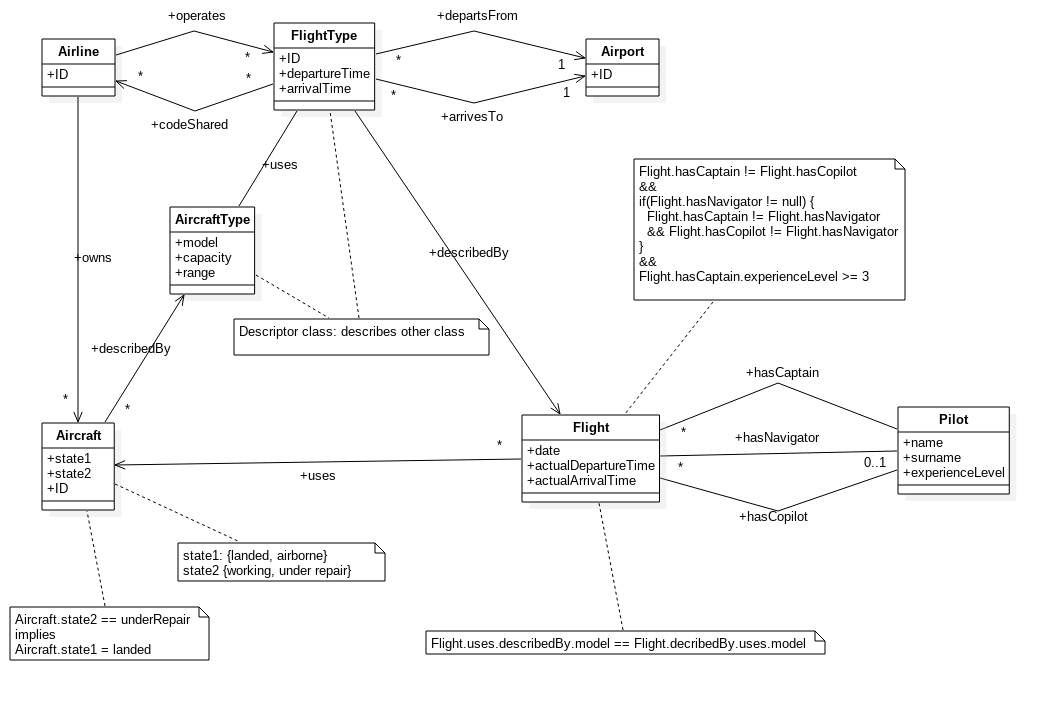
\includegraphics[scale=0.5]{exercises/classDiagram_flights.png}
\caption{Flights - Class Diagram}
\end{sidewaysfigure}
\chapter{User Interface design}
User interface design is more important for consumer and enterprise market with respect to embedded market. 

User interface is the portion of the system interacting with the user and, nowadays, three user interfaces are possible: web, desktop and mobile.

% Complexity of usage, Complexity of structure, Complexity of functions

\paragraph{Principles and ideas}
\begin{description}
\item [Ergonomy] Safety, adaptability, comfort, usability, \dots
\item [Emotional design] Beyound ergonomy, the interaction should cause positive emotions in the user;
\item [User experience] Usability + feelings + emotions + value;
\item [Transparent technology] No emphasis on technology, emphasis on interaction;
\item [Feedback, user centered design] No decision based on personal opinions, but feedback from real users.
\end{description}

\section{User centered design}
\begin{enumerate}
\item Identify the users
\begin{description}
\item [Personas] Identify and describe typical user representative of a class of users. For each persona describe life scenarios and for each persona or scenario identify possible interaction with application or object.
\end{description}

\item Define requirements
\begin{description}
\item [Focus group] A moderator starts and monitors discussion of a group of homogeneous people on a defined topics. The discussion can be open or script guided. This technique is dynamic and very productive but long.
\item [Questionnaires] Written questions with open or close answers. This technique provides a strict and statistical analysis which cover more data points.
\item [Interviews] Deep discussion, open or guided by script or questions, one to one reporting log. This technique provides a detailed analysis but requires a very long time.
\item [Ethnographics] Researcher is hidden in an environment and observes facts and behavior of the user and the population. This technique is expensive, long and risk of being invasive must be considered.
\end{description}

\item Define system and interactions
\begin{description}
\item [Prototypes] Low fidelity (sketches, post its) or high fidelity (computer executable mock ups). 
\end{description}

\item Feedback
\begin{description}
\item [A/B test] Try some variations of the user interface on a group of users and measures are taken, i.e.\@ how many users achieve the goal. 
\end{description}
\end{enumerate}
\chapter{Architecture and design}
Requirements show what the system should do. \emph{Architecture and design} show \textbf{how} the system should be built. Architecture and design have the same flavour but they focus on different levels:
\begin{itemize}
\item Architecture stands at high level and handles decisions about major components and communication framework;
\item Design stands at lower level and handles decisions about internal structure of each component.
\end{itemize}
Most defects come from requirements and design, therefore it is essential to define, analyze and evaluate design choices early. If no design is defined, but code is immediately developed, choices are made implicitly and evaluate later. Doing design allows to make design choices \emph{explicit}, document and evaluate them. Given a set of requirements, in general, many different designs are possible corresponding to different design choices, but not all designs are equal. Transforming requirement to design is a creative process driven by skill and experience formalized in semi formal guidelines, i.e.\@ architectural styles (patterns) and design patterns.

Design has two sides:
\begin{itemize}
\item \textbf{System design}: decisions about computing nodes and their connection. For embedded systems it includes also decisions about components and connections in other technologies, i.e.\@ electrical, electronic, mechanical, etc.
\item \textbf{Software design}: decisions about software components and their connections, within a given system design.
\end{itemize}

\section{Process}
\begin{enumerate}
\item Architecture
\begin{itemize}
\item Define high level components and their interactions;
\item Select communication and coordination model
\item Use architectural styles or patterns;
\end{itemize}
\item Design
\begin{itemize}
\item High level, about many classes: define classes and their interactions using design patterns;
\item Lowe level, about one class.
\end{itemize}
\end{enumerate}

\subsection{Design}
Definition of classes can be done exploiting glossary or context diagram and considering design patterns.
From glossary, it is needed to consider a class for each key entity in glossary, while from context diagram it is needed to consider a class for each actor, i.e.\@ physical device or subsystem and define GUI for each human actor.

Low level design concerns a single class or two. For each attribute, define type and privacy. For each method, define return type, number and type of parameters, privacy and choose an algorithm if needed. Possibly define getters and setters. For each relationship with other class, choose an implementation. Persistence must be decided, too.

\paragraph{Relationship}
Relationships are not directly implemented in most programming languages. Representing a relationship is a design choice depending of the direction of the arrow, references, list, etc.

\section{Properties}
Properties are split in two categories:
\begin{itemize}
\item \textbf{Functional properties}: does the design support the functional requirements?
\item \textbf{Non functional properties}: does the design support the non functional properties?
\begin{itemize}
\item Reliability;
\item Efficiency/performance;
\item Usability;
\item Maintainability;
\item Portability;
\item Safety;
\item Security;
\end{itemize}
and some more specific to design:
\begin{itemize}
\item Testability (observability, controllability);
\item Monitorability;
\item Interoperability;
\item Scalability;
\item Deployability;
\item Mobility;
\item Complexity (number of components, number of interactions);
\item Coupling or decoupling (degree of dependence between two components);
\item Cohesion (degree of consistence of functions of a component);
\item Cost;
\item Schedule;
\item Staff skills.
\end{itemize}
\end{itemize}

\begin{description}
\item [Performance] Localize critical operation and minimize communications. Use large rather than fine-grain components.
\item [Security] Use a layered architecture with critical assets in the inner layers.
\item [Safety] Localize safety-critical features in a small number of sub-systems.
\item [Availability] Include redundant components and mechanism for fault tolerance.
\item [Maintainability] Use fine-grain, replaceable components.
\end{description}
Using large-grain components improves performance but reduces maintainability. Introducing redundant data improves availability but makes security more difficult. Localizing safety-related features usually means more communication, hence degraded performance.

\paragraph{Tradeoffs}
Not all properties can be satisfied. Design is also about deciding tradeoffs, which possibly are decided at requirement time.

\section{Notations for formalization of architecture}
\subsection{Informal}
\paragraph{Box and line diagrams}
Very abstract technique. Boxes and lines do not  show the nature of component relationships nor the externally visible properties of the subsystems. However, this technique is useful for communication with stakeholders and for project planning.

\subsection{Semiformal}
\paragraph{UML diagrams}
They provide a structural view of component:
\begin{itemize}
\item Component or package diagram for high level view;
\item Class diagram, inside each package or component;
\item Class description, for each class.
\end{itemize}
UML helps in presenting structure in an organized and hierarchical way. UML can provide a dynamic view, too by using sequence diagrams which represent the sequence in which functions are called, as shown in figure~\ref{sequence_diagram}.

\begin{figure}[hbtp]
\centering
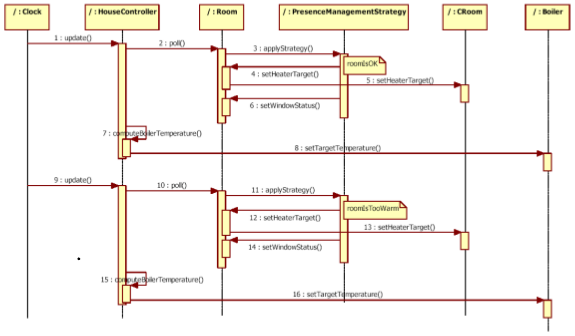
\includegraphics[scale=0.4]{images/uml_sequence_diagram.png}
\caption{Sequence diagram}
\label{sequence_diagram}
\end{figure}

\section{Patterns}
\emph{Patterns} are known and working ways of solving a problem. They provide reusable solutions to recurring problems in a defined context.

\subsection{Architectural patterns}
A real system is usually influenced by many architectural patterns.

\paragraph{Repository}
Subsystems must exchange data. When large amounts of data have to be shared, the repository model of sharing is the most commonly used. Sharing may be done in two ways:
\begin{itemize}
\item Shared data is held in a central database or repository and may be accessed by all subsystems;
\item Each subsystem maintains its own database and passes data explicitly to other subsystems.
\end{itemize}

\subparagraph{Advantages}
\begin{itemize}
\item Efficient way to share large amounts of data;
\item Subsystems need to be concerned with how data is produced;
\item Centralized management e.g.\@ backup, security;
\item Sharing model is published as the repository schema.
\end{itemize}

\subparagraph{Disadvantages}
\begin{itemize}
\item Subsystems must agree on a repository data model, which is inevitably a compromise;
\item Data evolution is difficult and expensive;
\item No scope for specific management policies;
\item Difficult to distribute efficiently.
\end{itemize}

\paragraph{Client-server model}
Distributed system model which shows how data and processing is distributed across a range of components. A set of stand-alone servers providing specific services can be accessed by a set of clients which can call these service, through a network which allows clients to access servers.

\subparagraph{Advantages}
\begin{itemize}
\item Distribution of data is straightforward;
\item Makes effective use of networked systems. May require cheaper hardware;
\item Easy to add new servers or upgrade existing servers.
\end{itemize}

\subparagraph{Disadvantages}
\begin{itemize}
\item No shared data model to subsystems using different data organization. Data interchange may be inefficient;
\item Redundant management in each server;
\item No central register of names and services. Finding out what servers and services are available may be hard.
\end{itemize}

\textbf{Abstract machine model} is used to model the interfacing of subsystems. It organizes the system into a set of layers, i.e.\@ abstract machines, each of which provide a set of services in such a way that a layer uses only services from adjacent layers.

In design, each layer is about a problem, i.e.\@ separation of concerns. In evolution, when a layer interface changes, only the adjacent layer is affected. The main problem is that sometimes is artificial to structure systems in this way.

\paragraph{Pipes \& Filters}
This technique is useful when data streams have to be processed according to several steps in a sequential way. It must be possible to recombine steps, taking into account that non-adjacent steps do not share any information and that the user storing data after each step may result into errors and garbage.

\paragraph{Other techniques}
Other possible techniques to use are layers, broker, MVC and microkernel.

%\subsection{Design patterns}
%\subsection{Idioms}

\section{Verification}
\emph{Verification} must check both functional and non functional requirements.

\subsection{Functional requirements}
\paragraph{Traceability matrix}
Each functional requirement must be supported by at least one function in one class in the software design. The more complex the requirement, the more member functions needed.

\paragraph{Scenarios}
Each scenario must be feasible. It is possible to define a sequence of calls to member functions of classes in the software design that matches the scenario.

\subsection{Non functional requirements}
Non functional requirements concern mostly of performance. Thus, scenarios are enriched with time model.

\subsection*{Bicycle example}
\paragraph{Functional requirements}
Transport one person from place to place.
\begin{itemize}
\item Steer;
\item Accelerate;
\item Brake.
\end{itemize}

\paragraph{Non functional requirements}
\begin{itemize}
\item Efficiency: speed from 10 km/h to 50 km/h, weight between 10 and 15 kg, reasonable torque to start (< 40 Nm);
\item Usability: out of 50 average users, at least 60\% of them find the bicycle easy to use;
\item Only human power, no engine;
\item Safety, no harm to driver;
\item Security, difficulty to steal;
\item Cost, between 100 and 200 euros.
\end{itemize}

\paragraph{Design vs requirements}
\begin{center}
\begin{tabularx}{\textwidth}{X|XXX}
 & Draisine & Velocipede & Dominant design \\ 
\hline 
Transport one person & Y & Y & Y \\ 
\hline 
Speed & < 10 km/h & Y & Y \\ 
\hline 
Torque at start & Y & N & Y \\ 
\hline 
Weight & Y & Y & Y \\ 
\hline 
Human power & Y & Y & Y \\ 
\hline 
Safety & Driver less high & Driver very high & Y \\ 
\hline 
Reduce speed & Feet on road & Negative force to pedal & Brakes \\ 
\end{tabularx}
\end{center}
\chapter{Configuration management}
A software is made of many parts (i.e.,\@ documents, programs, etc.) with different instances (customer, platforms, etc.) and thousands of separate documents are generated for a large software system. A software system changes because of different instances of software for different customers and because the same software changes over time.

Therefore, it is needed to identify the history of a document (versioning), the correct set of documents for a specific need (configuration), who can access and change what (change control) and how the system is obtained (build). \emph{Configuration management} permits to identifiy and manage parts of software, control access and changes to parts and allow to rebuild previous version of software.

\section{Versioning}
\emph{Versioning} permits to keep track of versions using same names or different version names in such a way that a user decides when to change version (commit operation) and that is always possible to recover a past version.

\paragraph{Configuration item}
A \emph{configuration item} (CI) is an element under configuration control. It is characterized by a name and a version number and all its version numbers are kept. The user decides to change version number with specific operation (\textbf{commit}) and it is possible to retrieve any version.

It is the basic unit for the configuration management system, e.g.,\@ a work product or piece of software that is treated as a single entity for the purpose of configuration management. It may correspond to one or more documents or one or more programs.

Not all documents in a project become a configuration item. If all documents are considered configuration items, a large overhead is introduced but, on the other hand, if no document is considered configuration item, no history is available and there is no information on configurations.

\paragraph{Configuration}
Configuration items have depencencies among them, some a re syntactically defined (e.g.,\@ \texttt{\#include} or \texttt{import} statements) but most are not, such as requirement and test cases. This requires a way to treat sets of configuration items, i.e.,\@ \emph{traceability}.

\begin{figure}[hbtp]
\centering
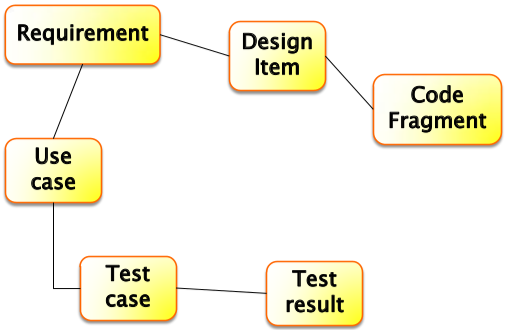
\includegraphics[scale=0.3]{images/dependency_traceability.png}
\caption{Dependency and traceability}
\end{figure}

A \emph{configuration} is defined as a set of items, each in a specific version and, generally, it includes not only source code. The same configuration item may appear in different configurations. Therefore, also a configuration has its version. There are two main approaches to identify a configuration:
\begin{enumerate}
\item ID for configuration, ID for configuration item: CVS;
\item ID for configuration, same ID for all configuration items in the configuration: Subversion, Git.
\end{enumerate}

\subparagraph{Approach 1}
Configuration items numbering and configuration numbering are independent. In this way, it is clear when a configuration item changes but the name of configuration item and configuration are managed separately.

\begin{figure}[hbtp]
\centering
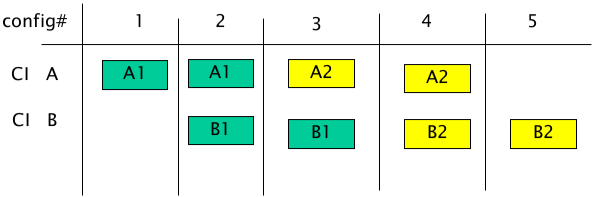
\includegraphics[scale=0.3]{images/configuration_approach1.png}
\caption{Configuration - Approach 1}
\end{figure}

\subparagraph{Approach 2}
Configuration number changes on every change. Items inherits the configuration numbering. In this way, configuration items and configuration are managed together, therefore it is unclear when a configuration item changes.

\begin{figure}[hbtp]
\centering
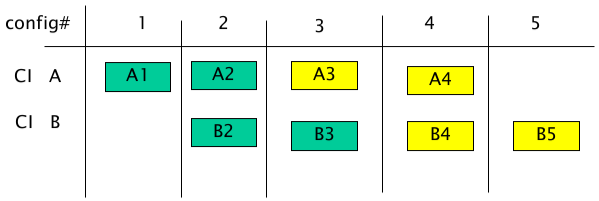
\includegraphics[scale=0.3]{images/configuration_approach2.png}
\caption{Configuration - Approach 2}
\end{figure}

\paragraph{Version}
A \emph{version} is a particular instance of a configuration item at a certain point in time. Each instance as a unique number and each configuration has a unique number.

\paragraph{Baseline}
A \emph{baseline} identifies a configuration in a stable, frozen form. Not all configurations are baselines.

\section{Change control}
Typically, a team develops a software. Hence, many people need to access parts of software contained in a common repository (shared folder) in such a way that all can read and write documents and programs.

\begin{description}
\item [Repository] Place where configuration items and configurations are stored.
\item [Workspace] Place where users work, on copies of configuration items.
\end{description}

\begin{figure}[hbtp]
\centering
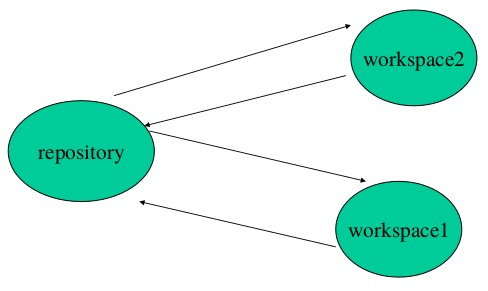
\includegraphics[scale=0.3]{images/repository_workspace.png}
\caption{Repository and workspaces}
\end{figure}

\subsection{Repository}
A \emph{repository} can implemented as a shared folder, containing shared files, on file server or using a CMS\footnote{Content Management System.} tool with change control (check-in, check-out). Changes must be disciplined, requiring knowledge about who controls, what is controlled and how control is implemented.

A repository can be implemented exploiting different approaches:
\begin{itemize}
\item Local: repository and user on the same machine;
\item Centralized: repository on a single server, many users (clients) can access and obtain copies of files;
\item Distributed: repository mirrored on all servers/clients.
\end{itemize}

\begin{description}
\item [Check-out] Extraction of configuration items from repository with purpose of changing it or not. After checkout. next users are notified.
\item [Check-in] Insertion of configuration items under control.
\end{description}

\begin{center}
\begin{tabularx}{\textwidth}{X|X}
\textbf{Check in/out} & \textbf{File system} \\
\hline
Configuration items are in repository & Files are in shared directory \\
\hline
To read/write a configuration item, user needs to perform checkout & Any user can get copy of file, or work on original \\
\hline
After checkout, next user knows that configuration item is used by someone else & Users can work on copies of file without knowing that others are doing the same
\end{tabularx}
\end{center}

\paragraph{Scenarios}
\subparagraph{Lock modify unlock - Serialization}
One can change at a time. Thus, no parallel work and delays. Problems if locker forgets to unlock. As shown in figure~\ref{img:lock_modify_unlock}, first check out locks the file and no other checkouts are allowed until checkin.

\begin{figure}[hbtp]
\centering
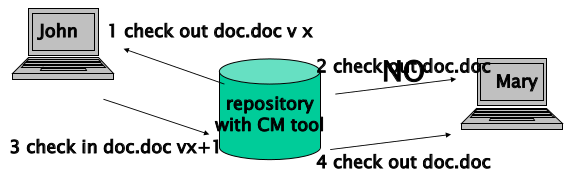
\includegraphics[scale=0.4]{images/lock_modify_unlock.png}
\caption{Lock modify unlock}
\label{img:lock_modify_unlock}
\end{figure}

\subparagraph{Copy modify merge}
Many change in parallel, the merge. It is more flexible but requires care to resolve possible conflicts. As shown in figure~\ref{img:copy_modify_merge}, the second check in signals conflict. User has to do manual merge of \emph{x+1} and \emph{x+1'} in \emph{x+2}.

\begin{figure}[hbtp]
\centering
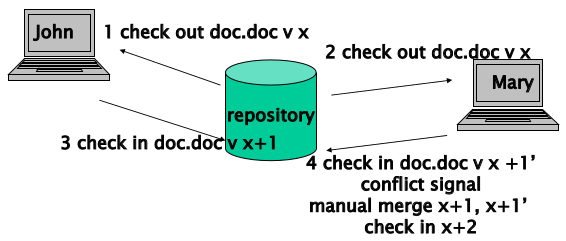
\includegraphics[scale=0.4]{images/copy_modify_merge.png}
\caption{Copy modify merge}
\label{img:copy_modify_merge}
\end{figure}

\paragraph{CMS approaches}
\begin{itemize}
\item Local: a simple database that kept all the changes to files under revision control, e.g.,\@ RCS;
\item Centralized: a single server that contains all the versioned files, and a number of clients that check out files from that central place, e.g.,\@ CSV, Subversion;
\item Distributed: clients fully mirror the repository, e.g.,\@ Git, Mercurial.
\end{itemize}

Very often, it is needed to proceed with \emph{parallel versions}, while keeping trace of common origin, as shown in figure~\ref{img:branches_merges}. For example, when some developers work on branch to fix defect, while other work to add functionalities.

\begin{figure}[hbtp]
\centering
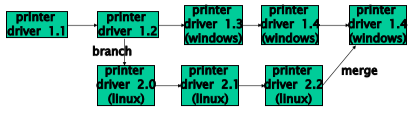
\includegraphics[scale=0.5]{images/branches_merges.png}
\caption{Branches}
\label{img:branches_merges}
\end{figure}

\paragraph{CM planning}
\emph{CM plan} contains key CM related choices and policies in a project, i.e.,\@ requirement and design documents, source files, test plan, test cases, configuration files, parameters, tools used in the production chain. It is needed to define which CM tool to use, what should and should not be a configuration item, control policies and who is the CM manager.

\paragraph{Build}
System \emph{building} is the process of compiling and linking software components into an executable system. Different systems are built from different combinations of components.

Systems are normally represented for building by specifying the filename to be processed by building tools. Dependencies between these are described to the building tools (e.g.,\@ Make, Ant, Maven). Mistakes can be made as users lose track of which objects are stored in which files. A system modelling language addresses this problem by using a logical rather than a physical system representation.

\begin{figure}[hbtp]
\centering
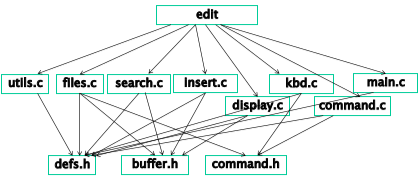
\includegraphics[scale=0.4]{images/dependencies.png}
\caption{Example of dependencies}
\end{figure}

\section{Git}
\subsection{Configuration management system}
A \emph{configuration management system} is a system that records changes to a file or set of files over time so that specific versions can be recalled later. Its functionalities are:
\begin{itemize}
\item Revert files back to a previous state;
\item Revert the entire project back to a previous state;
\item Compare changes over time;
\item Monitor who last modified something that might causing a problem;
\item Monitor who introduced an issue and when.
\end{itemize}

\paragraph{Data management models}
\begin{description}
\item [\textbf{Differences}] Information is kept as a set of files and the changes made to each file over time.
\item [\textbf{Snapshots}] Every commit, a picture of what all the files look like at a moment, is taken and the system stores a reference to that snapshot. If files have not changed, system stores just a link to the previous identical file.
\end{description}

\subsection{Introduction}
Git is a distributed CMS that uses snapshots. It exploits local operation and provides integrity. In fact, everything is check-summed before it is stored and is referred to by that checksum. No untracked changes of any file or directory are possible. Git only adds data. Each file has tree states:
\begin{itemize}
\item \textbf{Committed}: data is safely stored in local database;
\item \textbf{Modified}: the file has changed but it is not committed to the database yet;
\item \textbf{Staged}: a modified file is marked in its current version to go into next commit.
\end{itemize}

\begin{figure}[hbtp]
\centering
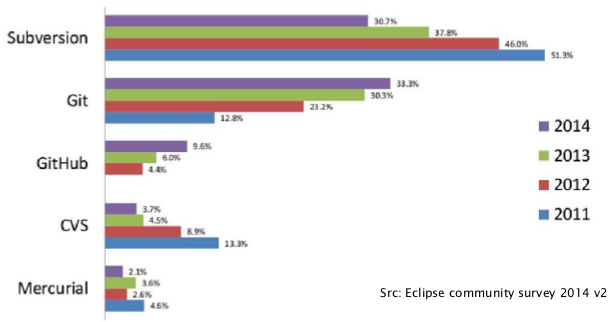
\includegraphics[scale=0.4]{images/cms_distribution.png}
\caption{CMS distribution}
\end{figure}

\paragraph{Sections}
\begin{description}
\item [\textbf{Git directory}] It stores the metadata and object database for the project. It is what is copied when a repository is cloned from another computer.
\item [\textbf{Working directory}] It is a single checkout of one version of the project. These files are pulled out of the compressed database in the Git directory and placed on disk to use or modify.
\item [\textbf{Staging area}] It stores information on what will go into next commit. Sometimes referred to as the \emph{index}.
\end{description}

\paragraph{Typical workflow}
\begin{enumerate}
\item Modify files in working directory;
\item Stage the files, adding snapshots of them to the staging area;
\item Do a commit, which takes the files as they are in the staging area and stores that snapshots permanently to the Git directory.
\end{enumerate}

\begin{figure}[hbtp]
\centering
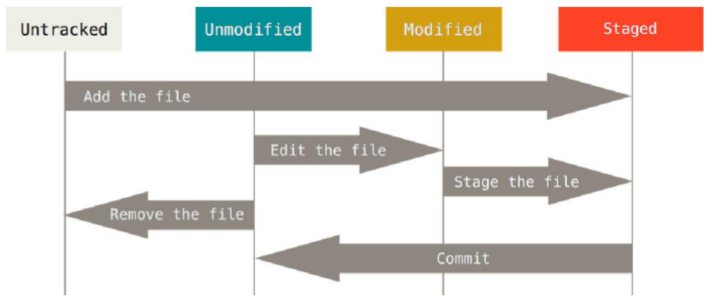
\includegraphics[scale=0.4]{images/file_lifecycle.png}
\caption{Lifecycle of files}
\end{figure}

\emph{Github} is an online code hosting service built on top of Git, mainly used by OSS projects but commercial use is growing. Nowadays, it is used by PayPal, SAP, vimeo and others.

\subsection{Basic commands}
\paragraph{Recording changes}
\begin{description}
\item [\texttt{git status}] determine which files are in which state.
\item [\texttt{git add}] track a new file.
\item [\texttt{git diff}] know exactly what is changed.
\item [\texttt{git commit}] commit changes.
\item [\texttt{git rm}] remove a file from the tracked files and also from the working directory.
\item [\texttt{git mv}] rename a file. Git doesn't explicitly track file movement. If a file is renamed in Git, no metadata is stored in it that tells the file has been renamed.
\end{description}

\paragraph{Commit history}
\begin{description}
\item [\texttt{git log}] look back to see what has happened in a repository.
\end{description}

\paragraph{Working with remotes}
\begin{description}
\item [\texttt{git pull}] automatically fetch and then merge a remote branch into your current branch.
\item [\texttt{git push}] share changes, i.e.,\@ transfer them on the server.
\end{description}

\subsection{Branching}
Git stores a commit object that contains a pointer to the snapshot of the context staged and pointers to the commit or commits that directly cam before this commits, i.e.,\@ its parent or parents. Staging the files, Git checksums each one, stores that version of the file (blobs) and adds that checksum to the staging area.

\paragraph{Branches}
A branch in Git is simply a lightweight movable pointer to commits. The default branch name in Git is \texttt{master}. Every commit, it moves forward automatically. \texttt{HEAD} pointer points to the current local branch.

Figure~\ref{img:git_branches} shows the status of commands:
\begin{enumerate}
\item \texttt{git branch testing} which creates a branch named \texttt{testing} but does not switch to that branch;
\item \texttt{git checkout testing} moves the \texttt{HEAD} pointer to that branch;
\item \texttt{git commit}.
\end{enumerate}

\begin{figure}[hbtp]
\centering
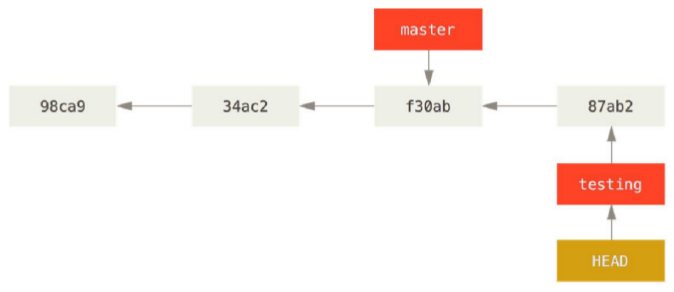
\includegraphics[scale=0.4]{images/git_branches.png}
\caption{Git branches}
\label{img:git_branches}
\end{figure}

\subparagraph{Switching branches}
Switching branches revert the files in working directory back to the snapshot that \texttt{master} points to. The changes made from this point forward will diverge from an older version of the project. Files in the working directory changes.

\subparagraph{Merging branches}
Figure~\ref{img:git_branches_merges} shows the status of commands:
\begin{enumerate}
\item \texttt{git merge hostfix} merges \texttt{hostfix} with \texttt{master}, assuming that current branch is \texttt{hostfix};
\item \texttt{git commit} on \texttt{iss53};
\item \texttt{git merge iss53} merges \texttt{iss53} with \texttt{master}.
\end{enumerate}
\begin{figure}[hbtp]

\centering
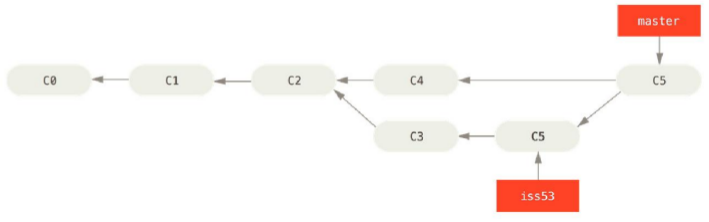
\includegraphics[scale=0.4]{images/git_branches_merges.png}
\caption{Git merge}
\label{img:git_branches_merges}
\end{figure}

Instead of just moving the branch pointer forward, Git creates new snapshot that results from this three-way merge and automatically creates a new commit that points to it. This is referred to as \emph{merge commit}, and is special in that is has more than one parent.

Git determines the best common ancestor to use for its merge base. Conflicts are possible, in this case merging is not done until conflicts are managed, as for commits.
\chapter{Verification \& Validation}
Validation is the task that verifies if the software system is the right one according to its effectiveness, external, i.e.\@  versus user, and reliability. Verification is the task that verifies if the software system is right according to its efficiency, internal, i.e.\@ correctness of vertical transformations, and correctness.

\paragraph{Scenario 1}
\begin{itemize}
\item Stakeholder
\begin{itemize}
\item Real need: big car with 6 seats.
\end{itemize}
\item Developers
\begin{itemize}
\item R1: compact car with 4 seats.
\item Result: compact car with 4 seats.

Verification passed, because the process is perfect for a compact car. Thus, translation from the requirement is ok.

Validation not passed, because of an error in the requirement which does not fit the stakeholder real need.
\end{itemize}
\end{itemize}

\paragraph{Scenario 2}
\begin{itemize}
\item Stakeholder
\begin{itemize}
\item Real need: big car with 6 seats.
\end{itemize}
\item Developers
\begin{itemize}
\item R1: big car with 6 seats.
\item Result: big car with 6 seats.

Verification passed.

Validation passed.
\end{itemize}
\end{itemize}

\paragraph{Scenario 3}
\begin{itemize}
\item Stakeholder
\begin{itemize}
\item Real need: big car with 6 seats.
\end{itemize}
\item Developers
\begin{itemize}
\item R1: big car with 6 seats.
\item Result: compact car with 4 seats.

Verification not passed.

Validation passed on requirement document, not passed on the product.
\end{itemize}
\end{itemize}

Requirements are the root of all evils. Validation is external because it involves users (actors) which have to check that their needs and their will have been respected.

\begin{figure}[hbtp]
\centering
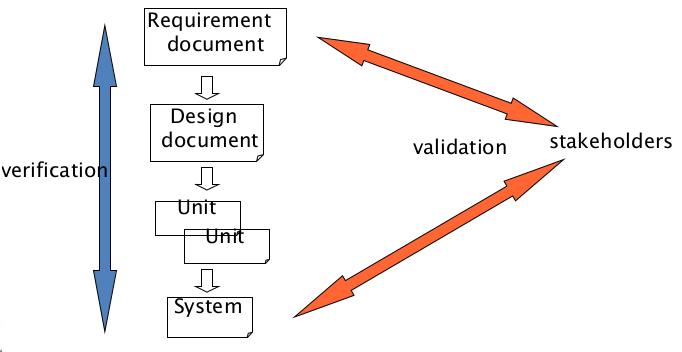
\includegraphics[scale=0.4]{images/v_v.png}
\caption{Verifican and Validation}
\end{figure}

Cost of fixing defect increases incredibly during the software process from the requirement document to the complete system.

\begin{description}
\item [Failure] An execution event where the software behaves in an unexpected way. Visible to the end user, who clearly knows that something is wrong.
\item [Fault] The feature of a software that causes a failure. May be due to an error in any part of the software, i.e.\@ incomplete/incorrect requirements, test cases, database, etc.
\item [Defect] Generally speaking, a failure or a fault. A defect is characterized by an insertion activity and (hopefully) a removal activity. In fact, some defects may never be removed because they are minor or too much difficult to fix. It is needed to always assume that there are some defects and minimize the discovering time. The idea is to find as much defect as possible before software release.
\end{description}

Verification and validation is an horizontal activity because it happens during the entire duration of software. Basic goals of verification and validation are:
\begin{itemize}
\item Minimize number of defects inserted, it cannot be zero due to inherent complexity of software;
\item Maximize number of defects discovered and removed;
\item Minimize time span between insertion and discover and removal.
\end{itemize}

\begin{figure}[hbtp]
\centering
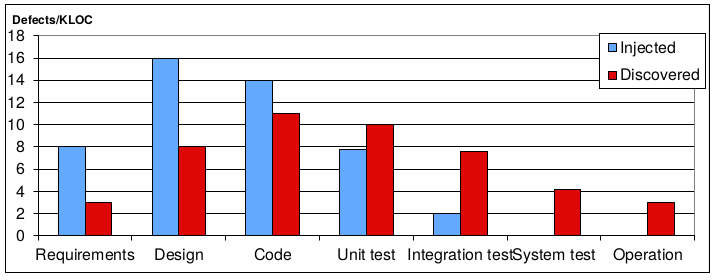
\includegraphics[scale=0.4]{images/defects_insertion_removal.png}
\caption{Insertion/removal by phase - Typical scenario}
\end{figure}

The longer the delay insert-remove, the higher the cost of removing defect. This is knows as \textbf{rework problem}, shown in figure~\ref{img:rework_problem} where red color represents a perfect process, with a bell shape, while yellow color represents actual rework which is more similar to an exponential.

\begin{figure}[hbtp]
\centering
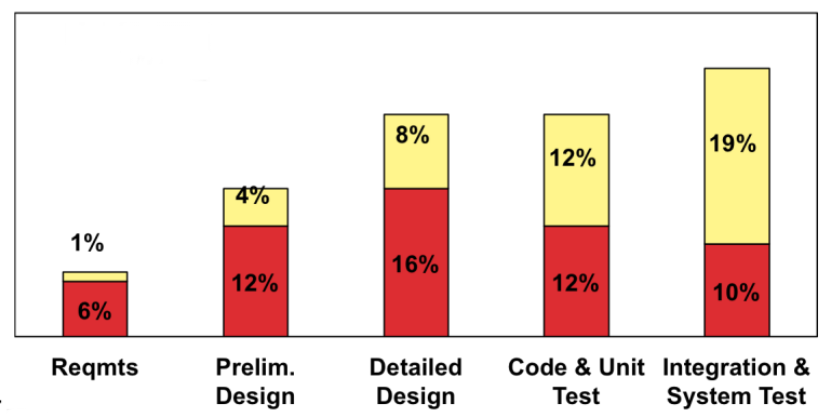
\includegraphics[scale=0.35]{images/rework_problem.png}
\caption{Rework problem}
\label{img:rework_problem}
\end{figure}

\section{Techniques}
\subsection{Static}
\subsubsection{Inspections}
\emph{Inspection} consist in reading documents and code by a group of people with goal of finding defects. Variants of inspections are reading techniques, walkthroughs or reviews. Many defects may be found, test phase concentrates one defect at a time.

\begin{figure}[hbtp]
\centering
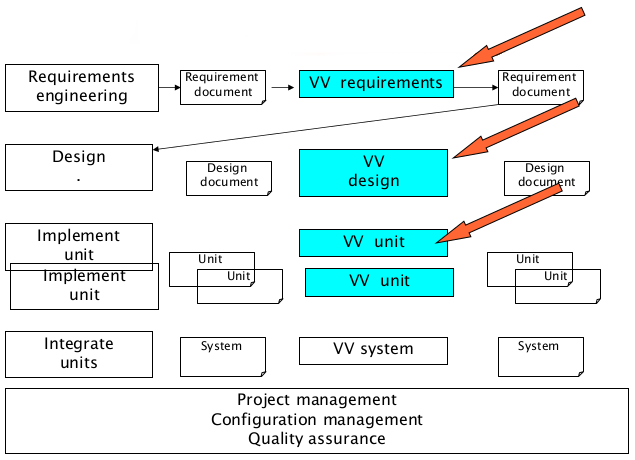
\includegraphics[scale=0.35]{images/v_v_inspection.png}
\caption{Inspection}
\label{img:v_v_inspection}
\end{figure}

This technique can be applied to documents and code. It is very effective because it reuses experience and knowledge of people on domain and technologies, it has more global and dynamic groups can be used. However, it is more suitable for functional aspects and it requires time, i.e.\@ effort and calendar time. Inspection and testing are complementary techniques and both should be used in V \& V.

Early defect detection improves product quality and reduces avoidable rework down to 10-20\%.

\paragraph{Roles in a group}
\begin{itemize}
\item \textbf{Moderator} leads inspection process and notably inspection meeting. It selects participants, prepares material. Usually, it is not from project that produces document to be inspected;
\item \textbf{Readers} read document to be inspected;
\item \textbf{Author} answers to questions that arise;
\item \textbf{Scribe} writes inspection log.
\end{itemize}

\paragraph{Fagan inspection process}
\begin{enumerate}
\item Planning: Select team, arrange materials, schedule dates;
\item Overview: Quickly present inspection group goals and document to be inspected;
\item Preparation: Important because inspectors are often unprepared. Read individually, applying inspection technique;
\item Inspection meeting: Team analysis to find defects. Group reads, discusses issues, agrees on problems. Scribe logs problems. Moderator keeps focus, keeps space, stops long discussions;
\item Rework: Author fixes defects/problem;
\item Follow-up: Repeat inspection or close and pass to next phase.
\end{enumerate}

Purpose of inspection is to find defects, not fix them. Group aims to produce best possible document avoiding ``kill the author'' game and ``relax and chat'' meetings.

\subsubsection{Technique vs. document}
\paragraph{Defect taxonomies for requirements}
Identify categories of common defects.

\begin{Parallel}{0.45\textwidth}{0.45\textwidth}
\ParallelLText{
One level
\begin{itemize}
\item Omission;
\item Incorrect fact;
\item Inconsistency;
\item Ambiguity;
\item Extraneous information.
\end{itemize}
}
\ParallelRText{
Two levels
\begin{itemize}
\item Omission
\begin{itemize}
\item Missing functionality;
\item Missing performance;
\item Missing environment;
\item Missing interface.
\end{itemize}
\item Commission
\begin{itemize}
\item Ambiguous information;
\item Inconsistent information;
\item Incorrect fact or extra functionality;
\item Wrong section.
\end{itemize}
\end{itemize}
}
\end{Parallel}

\paragraph{Checklist for requirements}
Based on past defect information. Questions refine a defect taxonomy.

\paragraph{Checklist for code}
Depends on programming language and on previous results of inspections.

\paragraph{Scenario-based reading}
Ask inspectors to create an appropriate abstraction which helps to understand the product. Ask inspectors to answer a series of questions tailored to the abstraction. Inspectors follow different scenarios each focusing on specific issues.

\paragraph{Defect-based reading}
A scenario-based reading technique to detect defects in requirements expressed in a formal notation. Each scenario focuses on a specific class of defects (data type inconsistency, incorrect functionality, ambiguity or missing functionality).

\paragraph{Perspective-based scenario} Widespread technique. A scenario-based reading technique to detect defects in requirements expressed in natural language, extended later for design and source code. Each scenario focuses on reviewing the document from the point of view of a specific stakeholder.

For each requirement and functional specification, generate a test or set of tests that allow you to ensure that an implementation of the system satisfies the requirement and functional specification. During the reading, the reader has to produce something, helping the reader to be careful and to keep focused.

\subsection{Dynamic}
\subsubsection{Testing}
\emph{Testing} is a dynamic technique that requires execution of executable system or executable unit. The purpose of testing process is to find defects in the software products, a test is successful if it reveals a defect. In fact, it is easy to show that something works being very soft in its usage.

Testing is also the process of operating a system or component under specified conditions observing or recording the results to detect the differences between actual and required behavior.

Defect testing and debugging are different activities, which may be performed by different roles in different times. Testing tries to find failures, while debugging searches for and removes the fault. Debugging, actually represent a short cycle of design and coding.

\begin{figure}[hbtp]
\centering
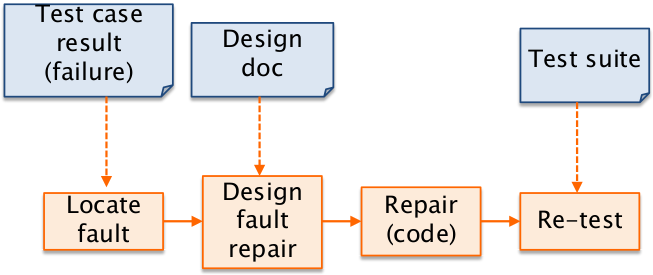
\includegraphics[scale=0.35]{images/debugging.png}
\caption{Debugging}
\end{figure}

A \textbf{test case} represents a stimulus applied to executable, system of unit, composed of name, input and expected output with defined constraints and context, e.g.\@ version and type of OS, DBMS, GUI, etc. \\
A \textbf{test suite} is a set of related test cases. \\
A \textbf{test case log} is composed by a test case reference, its time and date of application, its actual output and its result (passed or not passed).

Test activities:
\begin{enumerate}
\item Write test cases;
\item Run test case (test suite);
\item Record results.
\end{enumerate}

\begin{figure}[hbtp]
\centering
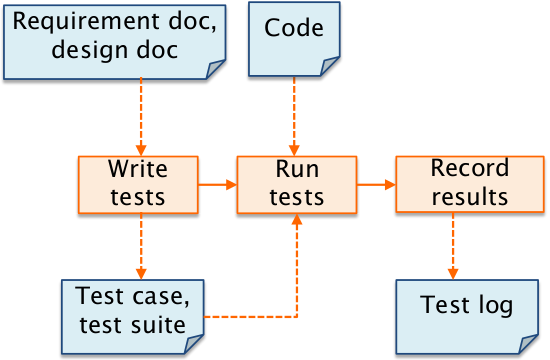
\includegraphics[scale=0.35]{images/test_activities.png}
\caption{Test activities}
\end{figure}

\paragraph{Possible scenarios}
\begin{enumerate}
\item Developer team and tester team are different. It is more complicated, longer and more expensive but it takes into account of different points of view, therefore more defects possibly arise;
\item Developer team both develops software and tests it. It is faster and cheaper but coverage is minor;
\item Developer team and tester team are different and after ``internal testing'', testing is repeated by a tester team (third party), possibly a certification authority, which ensures the quality. This approach is adopted in safety critical context.
\end{enumerate}

\paragraph{Oracle}
The ideal condition would be to have an automatic \emph{oracle}, very difficult to have, and an automatic comparator, available only is some cases. A human oracle is subject to errors. The oracle is based on the program specifications, which can be wrong. In order to perform testing, the expected behavior of a program for a given test case must be known.

A \emph{human oracle} is based on requirements specification or judgment.

An \emph{automatic oracle} is a model generated from formal required specification, e.g.\@ the same software developed by other parties or previous version of program (possibly leading to regression).

\begin{figure}[hbtp]
\centering
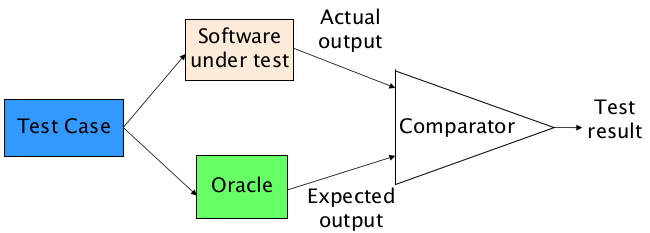
\includegraphics[scale=0.35]{images/oracle.png}
\caption{Oracle}
\end{figure}

\paragraph{Correctness}
\emph{Correctness}, in the sense of correct output for all possible input requires, exhaustive testing, which is unfeasible. Thus, goal of test are finding defects (not demonstrating that system is defect free) and assuring a \emph{good enough} level of confidence.

\subparagraph{Dijkstra thesis} Testing can only reveal the presence of error, never their absence.

\subparagraph{Weinberg's law} A developer is unsuitable to test his/her own code. Testing should be performed by a separate team or peers. If a developer misunderstand a problem, he cannot find such error.

\paragraph{Coverage} Test cases defined / Total test cases possible.

100\% and no failures $\Rightarrow$ correct.

\paragraph{Validity} A criterion is \emph{valid} if and only if whenever the produced output is incorrect, such a criterion selects at least one test set which is not successful for the output.

\paragraph{Reliability} A criterion is \emph{reliable} if and only if either every test selected by such a criterion is successful or no test selected is successful.

\subsection{Test classification}
\subsubsection{Testing per granularity level/phase}
\begin{itemize}
\item Unit tests: individual modules;
\item Integration tests: modules when working together;
\item System tests: the system as a whole, usable system.
\end{itemize}

\begin{figure}[hbtp]
\centering
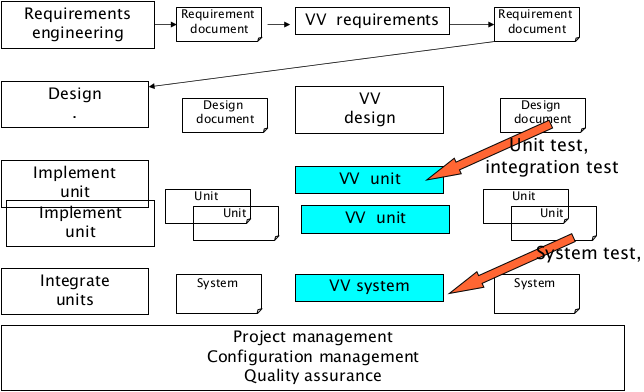
\includegraphics[scale=0.35]{images/testing_granularity_level.png}
\caption{Testing per granularity level/phase}
\end{figure}

\subsubsection{Testing per approach}
Given an object to test, approach can be
\begin{itemize}
\item Requirements driven: are the requirements of the object satisfied?
\item Structure: is the object built as it should?
\item Reliability: does it satisfy the customer need?
\item Risk: is it vulnerable to most likely risks?
\end{itemize}

\begin{table}
\centering
\begin{tabular}{|c|c|c|c|}
\hline 
\multirow{2}{*}{} & \multicolumn{3}{c|}{\textbf{Phase}} \\ 
\cline{2-4}
 & \textbf{Unit} & \textbf{Integration} & \textbf{System} \\ 
\hline 
\textbf{Functional (Black box)} & • & • & • \\ 
\hline 
\textbf{Structural (White box)} & • &  & \\ 
\hline 
\textbf{Reliability} & & & • \\ 
\hline 
\textbf{Risks} & & & • \\ 
\hline 
\end{tabular}
\caption{Testing classification}
\end{table}

\begin{table}
\centering
\begin{tabularx}{\textwidth}{|X|X|X|X|}
\hline 
 & \multicolumn{3}{c|}{\textbf{Testing phase}} \\ 
\hline
\textbf{Approach} & \textbf{Unit testing} & \textbf{Integration testing} & \textbf{System testing} \\ 
\hline 
\textbf{Requirements-driven} & 100\% unit requirements & 100\% product requirements & 100\% system requirements \\ 
\hline 
\textbf{Structure-driven} & 85\% logic paths & 100\% modules & 100\% components \\ 
\hline 
\textbf{Statistics-driven} & & & 90-100\% of usage profiles \\ 
\hline 
\textbf{Risk-driven} & As required & As required & As required \\ 
\hline 
\end{tabularx}
\caption{Testing classification and coverage}
\end{table}

\paragraph{Regression testing}
All test used in the past must be performed and no more defects must be found in a newer version.

\section{Unit test}
\subsection{Black box}
Black box testing is a functional test of units (functions, classes) which generates test cases starting from the specification of the unit. Source code is not needed.

\subsubsection{Random}
Random testing is independent of requirements but it requires many test cases. It is easy to define the inputs, but it requires an oracle to compute the expected output.

\subsubsection{Equivalence classes partitioning}
Input space is divided in partition that have similar behavior from the point of view of requirements for unit and a few test cases are performed for each partition. Boundary conditions must be defined to bound partitions and test cases are performed on the boundary, too.

\paragraph{Equivalence class} A class corresponds to set of valid or invalid inputs for a \emph{condition} on the input variables. If a test in a class has not success, the other tests in the same class may have the same behavior. Every equivalence class must be covered by a test case at least. Each test case for valid input classes must cover as many valid classes as possible.

\begin{enumerate}
\item Identify criteria, from requirements;
\item Define conditions for each criterion;
\item Define an order for combining conditions;
\item Combine conditions, identifying partitions;
\item Define one test case per partition.
\end{enumerate}

When a module has state, the state hast to be considered to define the partitions. State may be difficult to read/create and it requires a sequence of calls. Typically, object oriented classes have state and many functions have to be tested. Criteria and equivalence classes have to be identified and applied to each function.

\subsection{White box}
White box testing is structural and starts from the code, using several coverage objectives. White box testing is typically made in the development environment and supported by tools to compute coverage.

\paragraph{Statement coverage} Try to execute all statements in the program. \emph{Coverage} is a property of unit and test suite.
\[
\text{statement coverage} = \dfrac{\text{\# statements covered}}{\text{\# statements}}
\]

Problem is the concept of statement. Program can be transformed in \textbf{control flow}. A node represents an atomic instruction, i.e.\@ line terminated by a semicolon, or a decision, while an edge represents the transfer of control. Sequential nodes can be collapsed in a basic block. Statements which cannot be reached are called \emph{dead code}.

\emph{Control flow graph} makes more understandable which are basic (atomic) statements.

\paragraph{Node coverage} Evaluated for each test, considered cumulative for a test suite.
\[
\text{node coverage} = \dfrac{\text{\# nodes executed}}{\text{\# nodes}}
\]

\paragraph{Decision coverage} Try to cover all decisions in the program. Also called edge coverage because a decision corresponds to an edge in the control flow graph.
\[
\text{decision coverage} = \dfrac{\text{\# decisions covered}}{\text{\# decisions}}
\]

\paragraph{Relationships}
\begin{gather*}
\text{Node coverage} \Leftrightarrow \text{Statement coverage} \\
\text{Basic block coverage} \Leftrightarrow \text{Statement coverage} \\
\text{Edge coverage} \Rightarrow \text{Node coverage} \\
\text{Edge coverage} \nLeftarrow \text{Node coverage}
\end{gather*}

\paragraph{Condition coverage}
\begin{itemize}
\item Simple condition coverage: each condition is at least once true and at least once false, but the final decision may be the same;
\item Multiple condition coverage: all the combinations must be tested. It may not be feasible in some cases.
\end{itemize}

\begin{gather*}
\text{Multiple condition coverage} \Rightarrow \text{Decision coverage} \Rightarrow \text{Statement coverage} \\
\text{Multiple condition coverage} \Rightarrow \text{Simple condition coverage} \nRightarrow \text{Decision coverage}
\end{gather*}

\paragraph{Path coverage}
A \emph{path} is a sequence of nodes in a graph. Test cases should be selected in such a way that every path in the graph is visited. It may not be feasible, because of a combinatorial explosion with cycles. Some approximations are possible:
\begin{itemize}
\item Path-n: loop 0 to n times in each loop;
\item Loop coverage: in each loop cycle 0, 1, > 1 times.
\end{itemize}

\paragraph{Loop coverage}
Test cases should be selected such that every loop boundary and interior is tested:
\begin{itemize}
\item Boundary: 0 iterations;
\item Interior: 1 iteration and > 1 iterations.
\end{itemize}
Consider each loop separately and write three test cases: no enter the loop, cycle once in the loop, cycle ore than once.

\paragraph{Test representation}
\begin{description}
\item [Informal] Using keyboard or screen. No documentation of test case, nor test log.
\item [Formal] Programming languages.
\end{description}
Tools are provided to write and run test cases (e.g.\@ JUnit) and to compute coverage (e.g.\@ Cobertura).

\subsection{Mutation testing}
\emph{Mutation testing} consists in evaluating the goodness of test cases. The basic idea is to inject errors in program with single small change and to verify if test cases catch the injected errors. This approach is used both in software and hardware.

\begin{description}
\item [Mutant] Program with one change.
\item [Killable mutant] Non functionally equivalent. A test case can kill it.
\item [Equivalent mutant] Functionally equivalent. No test case can kill it.
\item [Mutation score] Property of a test suite, goal is 100\%.
\[
\text{mutation score} = \dfrac{\text{\# kiled non equivalent mutants}}{\text{\# non equivalent mutant}}
\]
\end{description}

\paragraph{Common mutations}
\begin{itemize}
\item Delete a statement;
\item Swap two statements;
\item Replace arithmetic operations;
\item Replace boolean relation;
\item Replace a variable;
\item Replace boolean sub-expression with constant value.
\end{itemize}

The main problem with mutation testing is time. In fact, many mutations are possible and a complete test suite is needed for each mutation.

\section{Integration testing}
Integration problems arise when more than one unit, possibly developed by different teams or in different time, interact together. In fact, it is possible that different conventions (i.e.\@ parameters order, parameter names, unit of measurement, etc.) have been used leading to unexpected results.

\begin{figure}[hbtp]
\centering
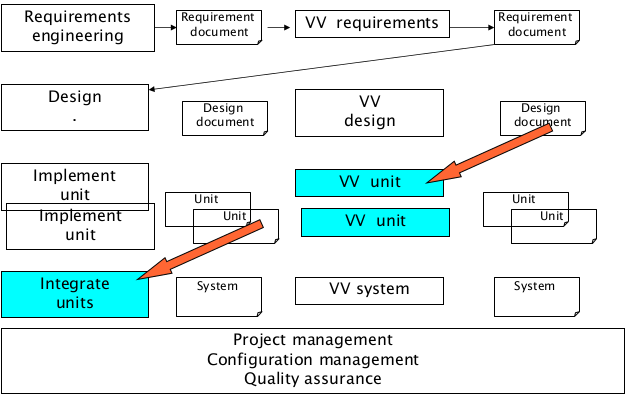
\includegraphics[scale=0.35]{images/integration_testing.png}
\caption{Integration testing}
\end{figure}

\paragraph{Dependency graph}
\emph{Dependency graph} shows dependencies among different units. It is useful to check if dependencies are correct.

\paragraph{Stub and driver}
A \emph{driver} is a unit (function or class) developed to pilot another unit. A \emph{stub} is a unit developed to substitute another unite, i.e.\@ fake unit. They are also called \textbf{mock ups}.

A stub must be simpler than the unit substituted, therefore it is needed to trade off simplicity and functionality, because a stub must be ``perfect'', i.e.\@ without defects.

\subsection*{Big bang integration}
Test is applied directly to the aggregate as if it was a single unit. This approach does not focus on the dependencies, therefore it is difficult to locate a defect when it is found. A defect can be generated by any function or by any interaction.

\subsection*{Test units in isolation}
Each unit is tested independently by using stubs or driver. It may be possible that writing stubs is a difficult and costly operation, which must be taken into account.

\subsection*{Incremental integration}
Goal is to add one unit at a time and to test the partial aggregate. In this way, when a defect is found, most likely, it comes by last unit/interaction added, but more test cases, stubs and/or drivers have to be written.

\paragraph{Top down}
\emph{Top down integration} allows to early detect architectural flaws because a limited working system (prototype) is available early, but it is suitable only for top-down development, requires the definition of stubs for all lower level units which are not directly observable.

\paragraph{Bottom up}
\emph{Bottom up integration} can start early in the development process and lower levels are directly observable, but it requires the definition of drivers for all lower level units.

\subsection*{Hardware software integration}
\emph{Hardware software integration} is suitable for embedded systems. Usually writing stubs for sensor or actuators implies defining a simulated model of the context of the software application, as defined by context diagram and system design.

\begin{enumerate}
\item Test software units with stubs replacing hardware;
\item Integrate software and hardware.
\end{enumerate}

\section{System testing}
\emph{System testing} is applied to the software system as a whole. It aims at verifying the correspondence of the system to the requirements. Typically it is not performed by the development team, but by a test team. Functional requirements are tested by covering uses cases as listed in the requirement document and considering usage profile, i.e.\@ typical ways of using the system. Test s performed in conditions as far as possible close to working conditions.

\begin{figure}[hbtp]
\centering
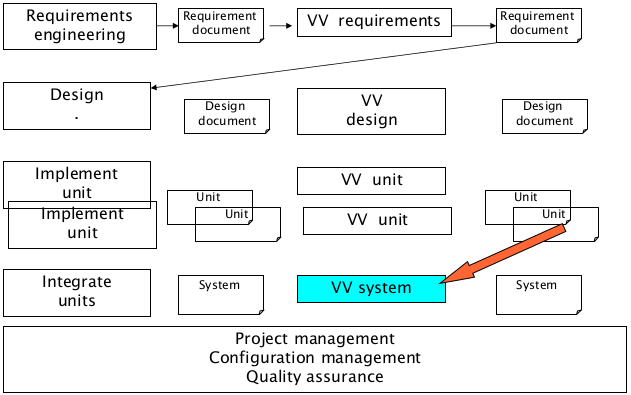
\includegraphics[scale=0.35]{images/system_testing.png}
\caption{System testing}
\end{figure}

\paragraph{Platform} The \emph{platform} is the environment where an application runs, defined by operating system, database, network, memory, CPU, libraries, etc.

An element can be tested on
\begin{itemize}
\item Target platform: where the element will run for day by day use. It cannot be used for production because data may be corrupted and it may not be available;
\item Production platform: where the element is produced. It cannot be, in most cases, equal to the target platform.
\end{itemize}
For an embedded system, production platform is typically a PC, with simulated/emulated external devices, while for an information system, is typically a PC or a workstation, whit a replicated database in a simplified form.

\paragraph{Variants}
System testing can be performed by end user (beta testing) or developer on development or target platform. \emph{Acceptance testing} is made by the user, possibly on both development and target platforms. Typically, it considers data and test cases provided by the customer on target platform.

\medskip

System testing test non functional requirements, which are usually emerging properties, in many cases testable only when the entire system is available, e.g.\@ efficiency, reliability.

\paragraph{Non functional properties}
\begin{itemize}
\item Configuration: the commands and mechanisms to change the system;
\item Recovery: the capability of the system to react to catastrophic events;
\item Stress: reliability of the system under limit conditions, e.g.\@ huge number of users;
\item Security: resilience to non authorized accesses.
\end{itemize}

\begin{table}
\centering
\begin{tabular}{|c|c|c|c|}
\hline 
 & \multicolumn{3}{c|}{Phase} \\ 
\cline{2-4} 
 & Unit & Integration & System \\ 
\hline 
Functional (Black box) & • & • & • \\ 
\hline 
Structural (white box) & • & & \\ 
\hline 
Reliability & & & • \\ 
\hline 
Risks & & & • \\ 
\hline 
\end{tabular} 
\caption{Testing classification}
\end{table}

\paragraph{Reliability testing}
\emph{Reliability testing} aims at providing estimate of reliability, i.e.\@ probability of failure over a period of time. Other possible measures are $\text{defect rate} = \text{defect}/\text{time}$ or $\text{MTBF} = \text{time between defects}$. In order to estimate reliability, a large number of independent test cases are needed, and defect fix must not introduce other defect, i.e.\@ regression testing.

\begin{figure}[hbtp]
\centering
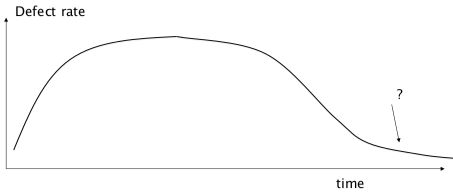
\includegraphics[scale=0.4]{images/software_reliability.png}
\caption{Software reliability}
\end{figure}

\paragraph{Risk based testing}
\begin{enumerate}
\item Identify risks;
\item Characterize risks: probability, effect;
\item Rank risks;
\item Handle risks.
\end{enumerate}

\paragraph{User profile based testing}
\emph{User profile based testing} is a variant of risk based testing:
\begin{enumerate}
\item Identify user profiles and usage profiles;
\item Rank them by frequency of usage;
\item Test more more used profiles.
\end{enumerate}
This approach is typically adopted on widespread software, e.g.\@ MS Word.

\paragraph{Regression testing}
Tests previously defined are repeated after a change to assure that the change has not introduced defects. In general, it is applied to all objects, i.e.\@ unit tests, integration tests and acceptance tests.

\begin{table}
\centering
\begin{tabularx}{\textwidth}{|X|X|X|X|X|}
\hline 
 & Functional / Non functional & Who tests & Platform & Techniques \\ 
\hline
\textbf{Unit test} & Functional / Structural & Developer or test group & Production  & BB, WB\\ 
\hline 
\textbf{Integration test} & Functional & Developer or test group & Production & Incremental~\footnote{Also called grey box, i.e.\@ internal testing but not so internal as white box.} TD or BU\\ 
\hline 
\textbf{System test} & Functional + Non functional & Developer or test group or user & Production, target & Requirement coverage, use case coverage \\ 
\hline 
\end{tabularx}
\caption{Testing}
\end{table}

\section{Documentation and automation}
%Non documenting test cases is a possible technique to perform informal and exploratory testing. 
Representing test cases can be done:
\begin{itemize}
\item Informally: reading is easy, but test cases are not executable, e.g.\@ Word document;
\item Formally:
\begin{itemize}
\item Word/Excel document and translator to programming language, e.g.\@ FIT, Fitness;
\item Programming language: executable and easily reusable (i.e.\@ regression testing) but less readable, e.g.\@ Eclipse + JUnit or similar.
\end{itemize}
\end{itemize}

Test cases should be documented, so that they are not lost and can be reapplied and automated, so that application of test cases is fast and error free.

\subsection{Testing tools}
\paragraph{Table based testing}
Test cases are written as tables in Word or Excel, and linked to application to be tested. In this way, end users are allowed to write tests, especially acceptance and black box ones, tests are independent of GUI and automation is possible. \emph{Fixtures} are needed to translate input from the table to the input of a coded function, to compare expected result to the actual one and to write the result. Using this approach, checking complex scenarios is difficult.

\paragraph{FIT framework for integrated testing}
Open source implementation of table based testing. User specifies tests in HTML tables, developer defines fixtures to parse tables and execute tests and Fit compares tables and actual results. \emph{FITnesse} is a standalone wiki allowing group to easily edit test files without worrying about ensuring the correct versions propagate out to all locations.

\paragraph{Coverage}
Show graphically and numerically coverage on source code, e.g.\@ Cobertura, Eclemma.

\paragraph{Profilers}
Trace time spent per function, given specific test execution, i.e.\@ performance test.

\subsubsection{GUI testing tools}
GUI testing is the practice of testing a GUI software through its user interface.
\begin{itemize}
\item \textbf{Functional testing}: black box tests exercising the basic functionalities of an application through interaction with the GUI, without knowing the source code;
\item \textbf{Look \& feel verification}: GUI should appear as defined in the requirements document, or in the mockups provided by the stakeholders.
\item \textbf{Compatibility testing}: testing that the application is deployed and behaving properly on different devices, screens and layouts (device diversity).
\end{itemize}

\paragraph{Approaches}
\begin{description}
\item [Manual] Manual execution of test scenarios.
\begin{itemize}
\item Easy to setup, does not require tools;
\item Error prone, hardly reproducible, expensive.
\end{itemize}
\item [Scripted] Development of test scripts using dedicated scripting languages.
\begin{itemize}
\item Scripts can be automatically executed and used for regression testing;
\item Test scripts can be difficult to write, and hard to maintain during the evolution of the software.
\end{itemize}
\item [Capture \& replay] User inputs are given once to the user interface (CAPTURE) and then codified into a repeatable script (REPLAY).
\begin{itemize}
\item Faster and easier to obtain test scripts with respect to pure scripted techniques;
\item Very fragile to the evolution of the user interface;
\item Script must be enriched manually to perform complex operations.
\end{itemize}
\item [Model-based] Test cases are obtained based on models of the user interface (e.g.\@ oriented graphs or finite state machines).
\begin{itemize}
\item Allow automated execution and generation of use cases;
\item Very high coverage of use cases and functionalities can be obtainable once a model is available;
\item Manual effort required in defining and tailoring the GUI model.
\end{itemize}
\item [Visual testing] Image recognition techniques are used to identify elements of the user interface to interact with.
\begin{itemize}
\item Easy definition of test cases with no need of technical knowledge - only screen captures are needed;
\item Can be applied seamlessly to any kind of software provided with an (emulated) user interface;
\item Very high fragility to even minor changes in the GUI;
\item Difficult in-depth testing of application functionalities.
\end{itemize}
\end{description}

\subsection{Test documentation}
\emph{IEEE Standard for Software Test Documentation} defines the deliverables to be produced by the testing process avoiding duplication between documents and between documents and tools.

\begin{figure}[hbtp]
\centering
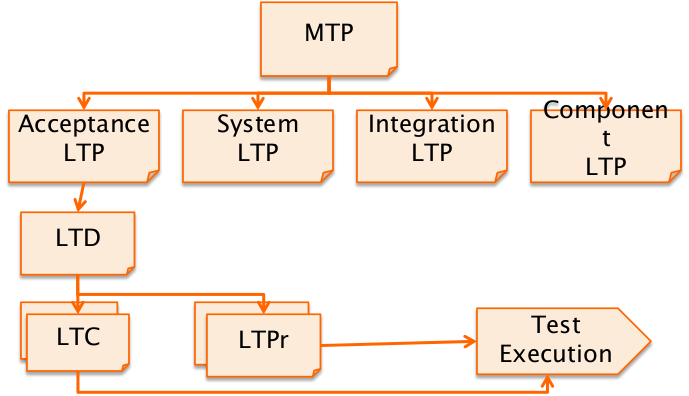
\includegraphics[scale=0.3]{images/deliverables.png}
\caption{Relationship among deliverables}
\end{figure}

\begin{Parallel}{0.45\textwidth}{0.45\textwidth}
\ParallelLText{
Planning and specification documents
\begin{itemize}
\item Master Test Plan;
\item Test Plan;
\item Test Design;
\item Test Case;
\item Test Procedure.
\end{itemize}
}
\ParallelRText{
Enactment documents
\begin{itemize}
\item Test Log;
\item Anomaly Report;
\item Interim Test Status Report;
\item Test Report;
\item Master Test Report.
\end{itemize}
}
\end{Parallel}

\paragraph{Master test plan}
\emph{Master test plan} guides the management of testing, establishes a plan and schedule, defines the required resources and generic pass/fail criteria, identifies the test items and explains the nature and extent of each test.

\paragraph{Level test plan}
\emph{Level test plan} defines testing activities (scope, approach, resources and schedule) and identifies items being tested, features to be tested, testing tasks to be performed, personnel responsible for each task and associated risks.

\paragraph{Traceability matrix}
\emph{Traceability matrix} maps tests to requirements and identifies which tests passed, and hence which requirements are satisfied. It may be part of test plan.

\paragraph{Test design specification}
\emph{Test design specification} specifies, for one or more features to be tested, the details of the approach, i.e.\@ testing techniques, analysis of results, list of test cases and motivation, generic attributes.

\paragraph{Test case specification}
\emph{Test case specification} specifies a test case in terms of goal, input data, expected output (oracle), test conditions (required hardware and software), special procedural requirements and inter-test dependencies. The test case is listed in a TDS document.

\paragraph{Test procedure specification}
\emph{Test procedure specification} specifies how to execute one or more test cases. The test procedure defines how to prepare the execution of the test, how to start and conduct the execution, which measurement to collect, how to suspend the test in presence of unforeseen events and how to resume a suspended test.

\begin{figure}[hbtp]
\centering
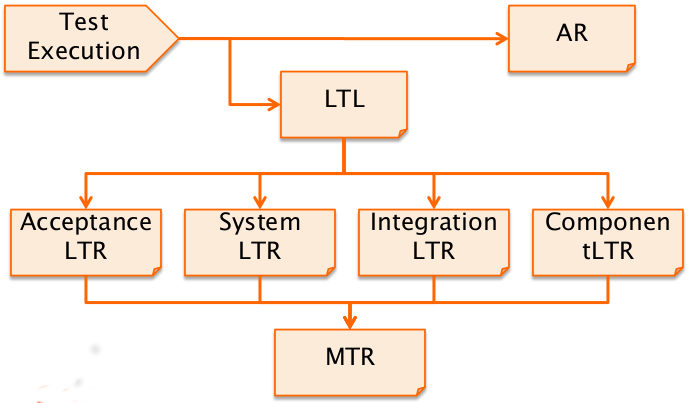
\includegraphics[scale=0.3]{images/deliverables_execution.png}
\caption{Execution deliverables}
\end{figure}

\paragraph{Execution deliverables}
Test item transmittal report which must describe a test item delivered for test and include at least identification of software item, its status and physical location. Test log, which must be a complete, systematic and chronological report of all details relative to test execution.

\paragraph{Level test log}
\emph{Level test log} provides a chronological record of relevant details about test execution. An automated tool may capture all or part of this information. It must include relevant info, i.e.\@ execution description, procedure results, environment and anomalies.

\paragraph{Anomaly report}
\emph{Anomaly report} documents any event that occurs during the testing process that requires investigation, including information about its time, its context, its impact and a description of input, expected and actual output and anomalies.

\paragraph{Interim test status report}
\emph{Interim test status report} summarizes the results of testing activities, including test status summary, changes from plans and test status metrics.

\paragraph{Level test report}
\emph{Level test report} summarizes the results of designated testing activities, including an overview of results, detailed results, i.e.\@ open and resolved anomalies, test executed and collected metrics and test assessment, and recommendations, i.e.\@ test items evaluation and suitability for production use.

\paragraph{Master test report}
\emph{Master test report} summarizes the results of all testing activities, including test tasks results, list of anomalies and resolutions, assessment of release quality and summary of collected metrics.

\section{Static analysis techniques}
This techniques are applied directly to the source code. Code is read by some tools without its execution.

\subsection{Compilation analysis}
Compilers analyze the code checking for syntax, types and semantic correctness. The errors detected by a compiler strongly depend on the language, e.g.\@ loose or strongly typed.

\paragraph{MISRA-C}
\emph{Motor Industry Software Reliability Association} defines some guidelines for C in order to limit possible but dangerous operations. For example:
\begin{itemize}
\item Use only character in the source character set. This excludes the characters \texttt{\$} and \texttt{@}, among others;
\item Declarations of identifiers denoting objects should the narrowest block scope unless a wider scope is necessary;
\item The operands of the \texttt{\&\&} and \texttt{||} operators shall be enclosed in parenthesis unless they are single identifiers;
\item Identifiers modified within the increment expression of a loop header shall not be modified inside the block controlled by that loop header;
\item Relational operators shall not be applied to objects of pointer type except where both operands are of the same type and both point into the same object.
\end{itemize}
Each rule probably helps to have a more reliable software. Source code is parsed, checking if rules are violated.

\paragraph{Bad smells}
Some indicators are specified to possibly detect issues. Mostly, these are design issues not strictly related to the code and they are not automatically recognizable by a tool, hence they have to be manually checked.

\begin{multicols}{2}
\begin{itemize}
\item Duplicated code;
\item Long method;
\item Large class;
\item Long parameter list;
\item Lazy class;
\item Message chain;
\item Middle man;
\item Incomplete library class.
\end{itemize}
\end{multicols}

\subsection{Data flow analysis}
\emph{Data flow analysis} analyzes the values of variables during execution to find out anomalies. It looks like dynamic but some information can be collected statically.
\begin{itemize}
\item Definition (write): a new value is assigned;
\item Use (read): the value of the variable is read;
\item Nullification: the variable has no significant value;
\end{itemize}
This approach is unfeasible in ``complicated'' code containing if-then-else or loop statements.

A \emph{correct sequence} is the one where the use of a variable is preceded by a definition of the same variable. A \emph{suspect/forbidden sequence} is the one where the use of a variable is not preceded by a definition. In fact, this corresponds to the use of an undefined value.

Some tools recover the sequence and recognize suspect ones.

\paragraph{Symbolic execution}
The program is executed with symbolic values instead of actual values. Output variables are expressed as symbolic formulas of input variables. Symbolic execution may be extremely complex even for simple programs.
\chapter{Software process models}
\emph{Software process models} define how to organize activities (e.g.,\@ requirement, design, \dots) and techniques that can be used to perform them (e.g.,\@ UML modelling, programming languages, testing, \dots).

\section{Phases and activities}
ISO/IEC 12207 defines how to identify processes, entities responsible of processes and products of each process. As shown in figure~\ref{img:iso_iec_12207}, the standard defines:
\begin{itemize}
\item Primary processes:
\begin{itemize}
\item Acquisition;
\item Supply;
\item Development;
\item Operation;
\item Maintenance.
\end{itemize}
\item Supporting processes:
\begin{itemize}
\item Documentation of product;
\item Configuration management;
\item Quality assurance:
\begin{itemize}
\item Verification \& Validation;
\item Reviews with customers;
\item Internal audits;
\item Problem analysis and resolution.
\end{itemize}
\end{itemize}
\item Organizational processes:
\begin{itemize}
\item Project management;
\item Infrastructure management:
\begin{itemize}
\item Facilities, networks, tools.
\end{itemize}
\item Process monitoring and improvement;
\item Training.
\end{itemize}
\end{itemize}

ISO 12207 only lists activities, independently of process model, technology, application domain and documentation.

\section{Process models}
A \emph{process model} defines how to organize activities, identifying roles, responsibilities, temporal constraints between activities satisfying constrains as laws or standards.

\subsection{Models}
Main constraints in defining a process model are:
\begin{itemize}
\item New development vs maintenance;
\item Compliance to standard or laws, related to criticality;
\item Size of end product, related with effort, calendar duration, size of staff involved, number and geographical distribution of teams.
\end{itemize}
Main operations in defining a process model are:
\begin{itemize}
\item Sequential vs parallel activities;
\item Iterations (a long one vs many short ones);
\item Emphasis or not on documents.
\end{itemize}

\paragraph{Build and fix}
\emph{Build and fix} model does not require any requirement, design or their validation. In fact, it is suitable only for solo programming and does not scale up for larger projects.

\paragraph{Waterfall}
\emph{Waterfall} [Royce 1970] is a document driven model which enforces sequential activities, each one producing a document used by the next one when the previous terminates.

It tends to use one long iteration, which is never feasible in practice because a change to a document implies re-doing all activities depending on it. Therefore, changes are long and expensive, leading to a lack of flexibility and tension to avoid changes.

Waterfall approach is suitable for large projects, distributed teams or contractors and mostly new developments where compliance is ensured by document. 

\begin{figure}[hbtp]
\centering
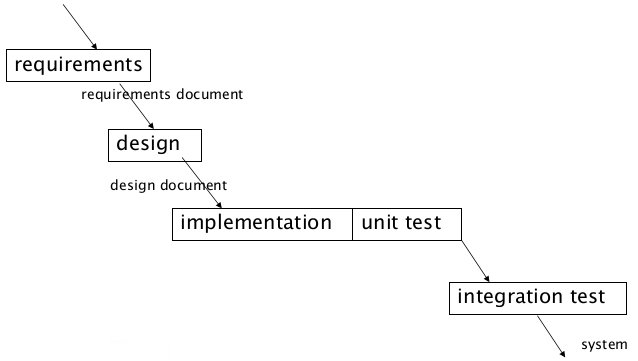
\includegraphics[scale=0.3]{images/waterfall_model.png}
\caption{Waterfall model}
\end{figure}

\emph{V model} is similar to waterfall, with emphasis on verification and validation activities. In fact, acceptance tests are written with requirements and unit or integration tests are written during design.

\paragraph{V model}
\begin{figure}[hbtp]
\centering
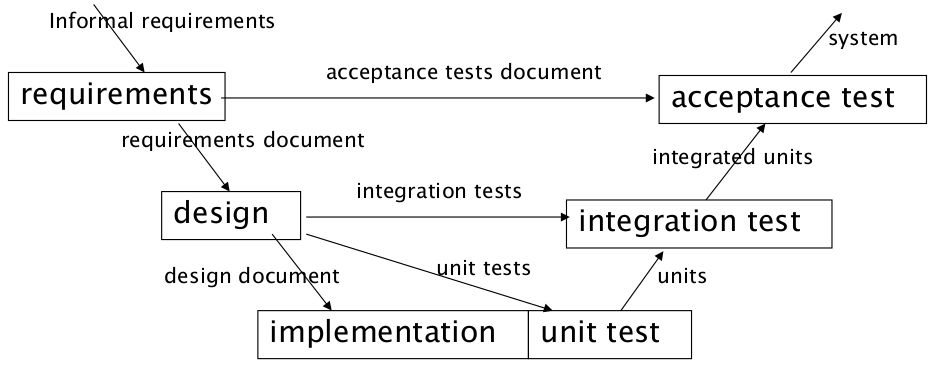
\includegraphics[scale=0.3]{images/v_model.png}
\caption{V model}
\end{figure}

\begin{figure}[hbtp]
\centering
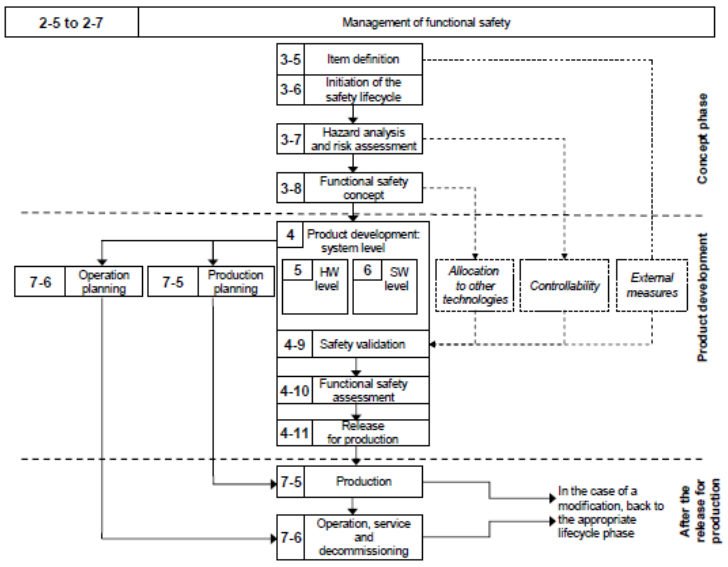
\includegraphics[scale=0.3]{images/safety_lifecycle.png}
\caption{Safety lifecycle}
\end{figure}

ISO 26262 and IEC 61508 are examples of V models. The first one is used in development of road vehicles requiring functional safety, which is an adaption of IEC 61508 used in safety industrial processes.

\begin{figure}[hbtp]
\centering
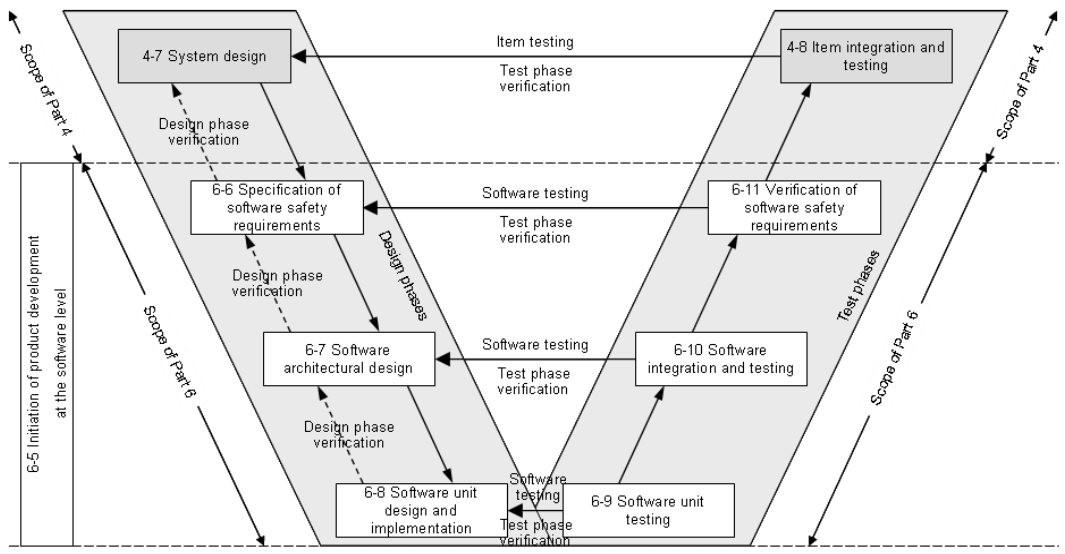
\includegraphics[scale=0.3]{images/software_lifecycle.png}
\caption{Software lifecycle}
\end{figure}

\paragraph{Prototyping}
\emph{Prototyping} consists of first building a quick and dirty prototype to validate and analyze requirements, then it is possible to proceed in a waterfall strategy. A software prototype is a product with less functions, possibly built in different platform, for instance a final embedded system produced in C can have a prototype written in Java or MATLAB emulated on a PC. The idea can be applied to other parts of a project, e.g.,\@ GUI prototyping, design prototyping, performance.

\begin{figure}[hbtp]
\centering
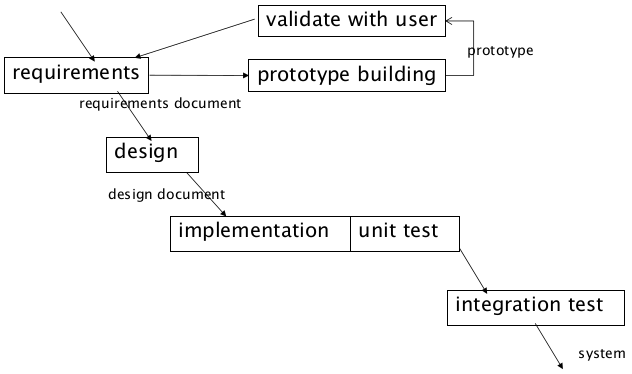
\includegraphics[scale=0.3]{images/prototyping_model.png}
\caption{Prototyping and waterfall model}
\end{figure}

In this way, it is possible to clarify requirements but this technique requires specific skills to build prototype, e.g.,\@ prototyping language and it would introduce business pressures to keep prototype, if successful, as final deliverable.

\paragraph{Incremental}
In waterfall, integration activity produces the complete system, that is delivered to costumer in one single shot. \emph{Incremental} model is the same as waterfall, but integration is split in such a way that every loop in integration produces a part of the system, therefore the system is delivered in several increments.

\begin{figure}[hbtp]
\centering
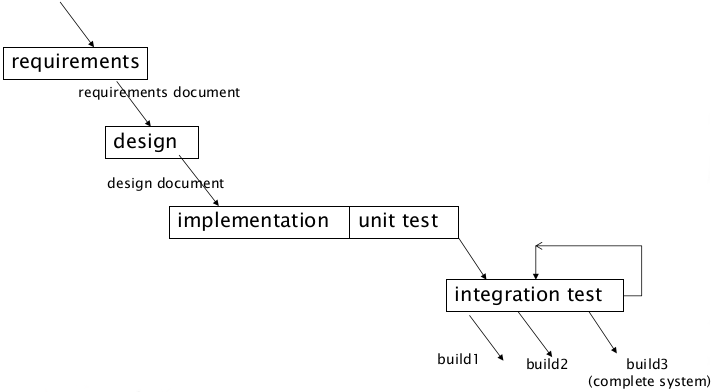
\includegraphics[scale=0.3]{images/incremental_model.png}
\caption{Incremental model}
\end{figure}

In this way it is possible to have an earlier feedback from user/customer and increments depending on external components can be delayed.

\paragraph{RUP}
\emph{Ration Unified Process} has been proposed in 1999. Activities are performed in parallel in one long iteration with sub-iterations exploiting a partial emphasis on documents. Iterations and deliveries (official releases) are planned and establish a point in time when everyone makes documents and code coherent and consistent with the others. In fact, this approach gives more flexibility and speed, but divergences are possible and must be limited.

\begin{figure}[hbtp]
\centering
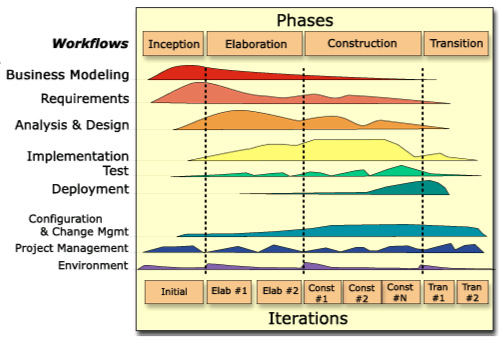
\includegraphics[scale=0.4]{images/rup_model.png}
\caption{RUP model}
\end{figure}

\begin{description}
\item [Inception] Feasibility study, risk analysis, essential requirements and possibly prototyping.
\item [Elaboration] Requirement analysis, architecture definition and project plan.
\item [Construction] Analysis, design, implementation and testing.
\item [Transition] Beta testing, performance tuning, documentation, training and packaging for shipment.
\end{description}
This approach is suitable for mostly new developments of possibly large projects, carried out by distributed teams, which require just partial compliance.

\paragraph{Reuse}
Most projects reuse components which can be open or closed source, free or not free. Therefore, availability is immediate, often with higher quality and lower cost but it leads to some issues like ownership of source, trade offs and loss of control on evolution.

It is needed to consider what is (un)available from components and change requirements accordingly. Components must be selected and evaluated, considering constraints and issues from components and adapt design consequently.

\begin{itemize}
\item Search and analysis of components;
\item Adaptation of requirements;
\item Design;
\item Implementation.
\end{itemize}

\subsection{Agile}
\emph{Agile} is a methodology where activities are performed in parallel in many short iterations without any emphasis on documents, i.e.,\@ just code and test cases, written as code.

This approach is suitable for both new developments on small projects and maintenance activities, carried out by co-located teams, without any compliance because no document is produced.

\paragraph{Agilemanifesto.org}
\begin{itemize}
\item Individuals and interactions over processes and tools;
\item Working software over comprehensive documentation;
\item Customer collaboration over contract negotiation;
\item Responding to change over following a plan.
\end{itemize}

\subsubsection*{Scrum}
\paragraph{Roles}
\begin{itemize}
\item Scrum master: Team leader;
\item Product owner: Stakeholder and business;
\item Development team: All activities, self organizing;
\end{itemize}

\begin{figure}[hbtp]
\centering
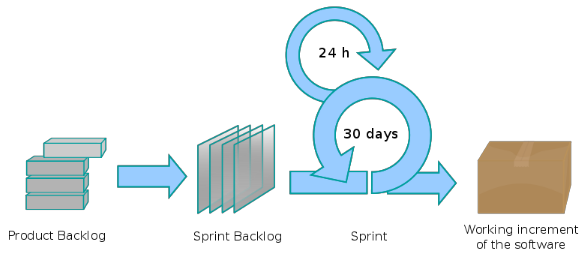
\includegraphics[scale=0.4]{images/scrum_process.png}
\caption{Scrum process}
\end{figure}

\paragraph{Documents}
\begin{itemize}
\item Product backlog: List of \emph{ordered} requirements for the product;
\item Sprint backlog: Requirements or activities for the sprint;
\item Increment: All what is done in all sprints. It must be usable.
\end{itemize}

\paragraph{Meetings}
\begin{itemize}
\item Daily scrum: Stand-up, 15 minutes;
\item Sprint planning meeting: One day;
\item Sprint reviewing meeting: Presentation to customer (demo), 4 hours;
\item Sprint retrospective (post mortem): Introspective.
\end{itemize}

\begin{table}
\centering
\small
\begin{tabularx}{0.95\textwidth}{X|X|X|X}
& \textbf{Waterfall} & \textbf{RUP} & \textbf{Agile} \\
\hline
\textbf{Activities} & Sequential & Parallel & Parallel \\
\hline
\textbf{Iterations} & One, long & One, long with sub iterations & Many, short \\
\hline
\textbf{Emphasis on documents} & Heavy & Mild & No \\
\end{tabularx}
\caption{Options}

\begin{tabularx}{0.95\textwidth}{X|X|X|X}
& \textbf{Waterfall} & \textbf{RUP} & \textbf{Agile} \\
\hline
\textbf{New development / Maintenance} & Mostly new development & Mostly new development & Both \\
\hline
\textbf{Compliance} & Yes & Partial & No \\
\hline
\textbf{Size} & Large projects, distributed teams and contractors & Also large projects, distributed teams & Small projects, co-located teams \\
\end{tabularx}
\caption{Suitability}
\end{table}

\subsection{eXtreme Programming}
The fundamental idea behind \emph{eXtreme Programming} is to have very short iterations with fast deliveries, by performing continuous testing and exploiting pair programming. eXtreme Programming is based on some basic facts:
\begin{itemize}
\item Producing code is required to deliver a system;
\item Money spent on analysis and design are wasted if the system is never used;
\item Business requirements have to be the drivers for software development;
\item Requirements change.
\end{itemize}
and requires four values:
\begin{itemize}
\item Communication: face to face, rather than document driven;
\item Simplicity: build a simple thing that should work;
\item Feedback: put system into production as soon as possible;
\item Courage: at every iteration it is possible to change many misunderstood or useless things.
\end{itemize}

\subsubsection{Practises}
\paragraph{On-site customer}
Real customer has to be part of the team, in order to define business needs, answer questions, resolve issues and prioritize features.

\paragraph{Small releases}
Put system into production as soon as possible in order to receive a fast feedback, delivering valuable features first in short cycle time, because planning 1-2 months is easier than planning 6-12 months.

\paragraph{Metaphor/Architecture}
Long documents may not be read by all people. Therefore, it is better to have a short description, i.e.,\@ metaphor, including few concepts which can be well understood, shared and agreed by all the people involved. Therefore, the initial architecture is actually a prototype of the final architecture.

\paragraph{Simple design}
The ``right'' design will run all tests, fulfills all current business requirements avoiding code duplication and using fewest possible classes and methods, remembering that design is made for today, not for the future.

\paragraph{Refactoring}
\emph{Refactoring} consists of restructuring the system without changing the functionality with the goal of keeping design simple, e.g.,\@ by changing bad design if found or removing dead code. Refactoring is useful to improve some non functional properties, e.g.,\@ maintainability, usability, performance by changing internal design.

From a business point of view, this is a useless procedure because, actually, it does not produce any delivery (functionality)

\paragraph{Pair programming}
All production code is written with two people looking at one machine and pairs change all the time. In this way, code is permanently inspected but it is possible that some development time is needed.

With respect to solo programming, quality should increase, duration should decrease and effort should increase, i.e.,\@ Pair programming favors quality, reduces duration and increases effort. Effect of group dynamics and skill of pairs must be considered, some guidelines are shown in table~\ref{tab:pp_guidelines}.

\begin{table}
\centering
\small
\begin{tabularx}{0.95 \textwidth}{|l|l|X|}
\hline
\textbf{Experience} & \textbf{Task complexity} & \textbf{Use of pair programming} \\
\hline
Junior & Easy & Yes, provided that increased quality is the main goal. \\
\cline{2-3}
 & Complex & Yes, provided that increased quality is the main goal. \\
\hline
Intermediate & Easy & No. \\
\cline{2-3}
 & Complex & Yes, provided that increased quality is the main goal. \\
\hline
Senior & Easy & No. \\
\cline{2-3}
 & Complex & No, unless you are sure that the task is too complex to be solved satisfactorily by an individual senior programmer. \\
\hline
\end{tabularx}
\caption{Guidelines for when to use pair programming}
\label{tab:pp_guidelines}
\end{table}

\paragraph{Test driven development}
Automatic test drivers. Test are written before code production from developers and customers, with a strong emphasis on regression testing in such a way that unit tests pass 100\% and the code is always under testing.

\paragraph{Planning game}
\begin{itemize}
\item Business decisions:
\begin{itemize}
\item Which ``stories'' should be developed;
\item Priority of stories;
\item Composition of releases;
\item Release dates. 
\end{itemize}
\item Technical decisions:
\begin{itemize}
\item Time estimates for features/stories;
\item Elaborate consequences of business decisions;
\item Team organization and process;
\item Scheduling.
\end{itemize}
\end{itemize}

\paragraph{Sustainable development}
Developing full speed only works with fresh people. Working overtime for two weeks in a row indicates problems.

\paragraph{Collective ownership}
All code can be changed by anybody on the team and everybody is required to improve any portion of bad code he/she sees. Individual code ownership tends to create experts.

\paragraph{Contiguous integration}
Integration happens after a few hours of development.Code is released into current baseline on integration machine and all test are run, possibly during the night or when the system is not ``stressed''. In case of errors, the previous version is restored and problems are fixed before the next release.

\paragraph{Coding standards}
In order to achieve collective ownership, teams has to adopt a coding standard which makes other people's code more understandable and avoids code changes because of syntactic preferences.

\paragraph{Environment}
The \emph{environment} has to support communication among developers, e.g.,\@ open space or common spaces. It is evident that the working environment has great influence on quality and quantity of work. Interruptions by colleagues, email or meetings and lack of comfort due to noise or light are negative factors.

\section{Maintenance process}
Change is the key element in a \emph{maintenance} process. A change can be
\begin{itemize}
\item A defect to be fixed (corrective maintenance); \item A modification to an existing function (perspective maintenance);
\item A new function (evolutive maintenance).
\end{itemize}
Changes can be originated by end users or developers and are received and processed by a group of maintainers.

The product evolves by applying a flow of changes, typically with regular releases which can be major, i.e.,\@ every few months, or minor/critical, i.e.,\@ when needed. The stable baseline is released regularly, while the working baseline is the one where maintainers work.

\paragraph{Process}
\begin{enumerate}
\item Receive change request;
\item Filter:
\begin{itemize}
\item Merge similar change requests;
\item Discard unfeasible or incorrect change requests;
\end{itemize}
\item Assess:
\begin{itemize}
\item Evaluate impact of change request in terms of effort/cost, feasibility, impact on architecture and/or functionality;
\item Rank change requests, using severity for the corrective ones and importance for the evolution ones;
\end{itemize}
\item Assign change request to a (team of) maintainer;
\item Implement change request
\begin{itemize}
\item Design, code, unit test, integration test;
\item System test;
\item Insert in next release.
\end{itemize}
\end{enumerate}
Only a part of change requests, even corrective, are actually implemented.

The flow of changes can radically change a product over time, therefore it is needed to control or maintain architecture in order to prevent architecture erosion and it is needed to control suitability for market and users.

\begin{figure}[hbtp]
\centering
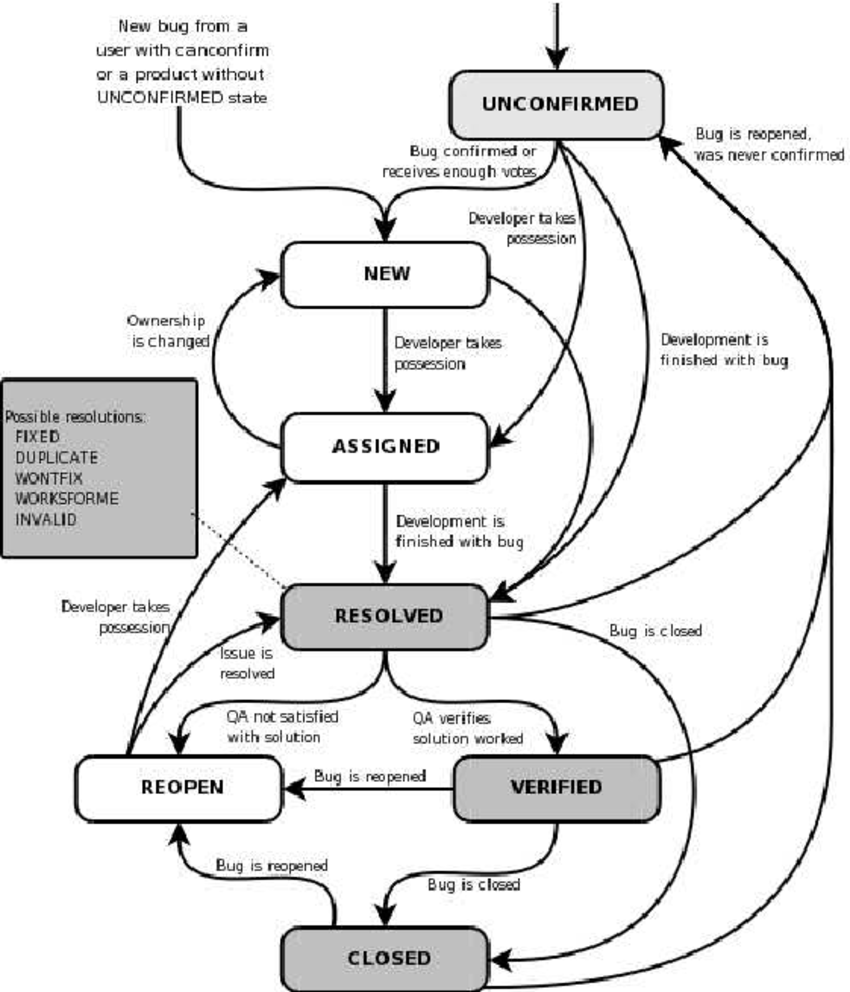
\includegraphics[scale=0.35]{images/bug_lifecycle.png}
\caption{Lifecycle for change (bug)}
\end{figure}

\section{Real cases}
\subsection{Ferrari}
\paragraph{Products}
\begin{itemize}
\item Electronic Control Unit ECU (embedded software):
\begin{itemize}
\item Power unit: engine, energy recovery;
\item Gearbox;
\item Brakes.
\end{itemize}
\item Support tools:
\begin{itemize}
\item Simulation of car;
\item Telemetry;
\item Configuration;
\item Pit stop control.
\end{itemize}
\end{itemize}

\paragraph{Process and toolchain}
\begin{enumerate}
\item Simulink model;
\item Translation to C;
\item Compilation to assembly;
\item Configuration and tuning;
\item Upload to firmware.
\end{enumerate}

\paragraph{Process and timing}
About two weeks between races:
\begin{itemize}
\item Requirements: 2 days;
\item Coding: 2 days;
\item Test: 4 days;
\item FIA freezing: 3 days;
\item Race: 3 days.
\end{itemize}
In one season, from March to November:
\begin{itemize}
\item 300 versions of embedded code;
\item 100 versions tools;
\item 1000 change requests, including few trivial bugs and tens of conceptual defects, i.e.,\@ requirement misunderstandings).
\end{itemize}
Issues are due to tight schedule and interaction among mechanical and software engineers.

\subsection{Apache}
\paragraph{Process}
Process is organized as an evolution/maintenance process spanning many years.
\begin{itemize}
\item Tools:
\begin{itemize}
\item CVS;
\item Mailing list;
\item Bugzilla (bug tracking).
\end{itemize}
\item Products:
\begin{itemize}
\item Source code;
\item Test cases;
\item Informal documentation (mails, bugs, comments).
\end{itemize}
\end{itemize}

\paragraph{Roles}
\begin{itemize}
\item Core team (2-8 people);
\item Patch developers (10-100 people);
\item Bug providers (100-1000+ people);
\item Others.
\end{itemize}

\paragraph{Facts}
\begin{itemize}
\item Limited documentation:
\begin{itemize}
\item No project plan, no quality plan, no requirement document.
\end{itemize}
\item Key points:
\begin{itemize}
\item Strict CVS;
\item Simple and effective tools for bug and change tracking;
\item Hierarchy of roles and responsibilities;
\item Motivated developers, especially in core team.
\end{itemize}
\end{itemize}

\subsection{Synchronize and Stabilize}
This approach was adopted by Microsoft from 1993 to 1995. It is a variant of the RUP and it is applicable in contexts where requirements can be fixed early on and it is needed to build complex products (millions of line of codes) with several interacting components, therefore with a design hard to devise and freeze early on.

\paragraph{Planning phase}
\begin{itemize}
\item Vision statement - Product managers:
\begin{itemize}
\item Define goals for the new products;
\item Priority order user activities that need to be supported by product features.
\end{itemize}
\item Deliverables:
\begin{itemize}
\item Specification document;
\item Schedule and ``feature team'' information:
\begin{itemize}
\item 1 program manager;
\item 3-8 developers;
\item 3-8 testers (1:1 ratio with developers\footnote{The idea is to spend half of the time for testing.}).
\end{itemize}
\end{itemize}
\end{itemize}

\paragraph{Development phase}
\begin{itemize}
\item Plan 3-4 subprojects (iterations) lasting 2-4 months each;
\item Buffer time between iterations;
\item Subprojects require design, code and debug, starting from the most critical features and shared components.
\end{itemize}

\subparagraph{Subproject development}
Feature teams go through the complete development cycle, feature integration, testing and fixing problems, synchronizing work by building the product, finding and fixing errors on a daily and weekly basis. Testers are paired with developers.

\paragraph{Stabilization phase}
\emph{Stabilization} requires testing (internal and/or external) and release preparation.

\subsection{Cyber physical ecosystems}
This approach is adopted by Wikipedia, Google, Twitter and in all products where a ``city model'' can be adopted:
\begin{itemize}
\item No clear boundary (APIs and mash ups);
\item Requirements are never known and emerge from individual contributions;
\item Continuous evolution without any release or planning;
\item Continuous operation without clear development and maintenance phases, always on and always changing;
\item Always ``beta'';
\item Emergent behaviors.
\end{itemize}

\paragraph{Structure}
\begin{itemize}
\item Core/Kernel providing horizontal functions: always on, top reliability, closed and slow to change. Requirements and architecture are well defined, controlled by core team; 
\item Periphery providing end user functions and content: fast changing, open. Requirements and design are unclear, unstable and crowdsourced without control.
\end{itemize}

\section{Process selection}
\paragraph{Process attributes}
\begin{itemize}
\item Sequential or parallel activities;
\item Iterations or no iterations;
\item Time framed or not;
\item Colocation of staff;
\item Emphasis on documents.
\end{itemize}

\begin{table}
\centering
\begin{tabular}{|l|l|l|l|l|}
\hline
& \textbf{Agile} & \textbf{26262} & \textbf{RUP} & \textbf{Sync Stab} \\
\hline
\textbf{Iteration number} & Many & One+ & Few & Few \\
\hline
\textbf{Iteration duration} & Weeks & Long & Months & Months \\
\hline
\textbf{Parallel activities} & Yes & No & Yes & Yes \\
\hline
\textbf{Documents} & Few & Many & Many & Few \\
\hline
\textbf{Colocation staff} & Yes & Yes or not & \multicolumn{1}{c|}{-} & Yes \\
\hline
\end{tabular}
\caption{Process comparison}
\end{table}

\subsection{Product attributes}
\paragraph{Criticality}
\emph{Criticality} defines emphasis on reliability, safety and security. Norms and laws may be applied, about legal responsibilities, too.

\paragraph{Size}
\emph{Size} can be evaluated in line of codes, in duration of development and team size or number of subcontractors. Size affects coordination and communication during development and maintenance.

\paragraph{Domain}
\emph{Domain} has effect on norms and laws applied, e.g.,\@ Basel~3 in finance, 26262 in automotive, and responsibility of developer, operator and maintainer.

\paragraph{Lifecycle}
Expected \emph{lifecycle} has effects on tradeoff development cost vs maintenance cost. Each lifecycle phase can be either a new development or a maintenance activity.

\paragraph{Bespoke or Market driven}
It has effect on time to market, requirement collection and ranking, cost structure and business model.
\begin{itemize}
\item Bespoke: one customer or end user;
\item Market driven: Many customers or end users.
\end{itemize}

\paragraph{Ownership}
\emph{Ownership} has effect on capability of modifying code, i.e.,\@ parametrization or adaptation. It can be full property, copyright, copyleft.

\paragraph{Relationship with developer}
\emph{Developer} can be the same as end user, an internal department of the company or an external company.

\subsection{Rules of thumb}
\begin{itemize}
\item Reliability, safety: waterfall-like (document based, few iterations, no parallel activities);
\item Market driven (time to market): frequent iterations;
\item Colocation of staff: if no, document-based and no parallel activities;
\item Size: the bigger, the more documents and activities;
\item Lifetime: if long, documents are required.
\end{itemize}

\appendix
\chapter{GUI Testing with Expresso}
\begin{table}
\centering
\begin{tabular}{|c|c|}
\hline 
GUI Graphics & Visual GUI Testing \\ 
\hline 
GUI Definition (XML files) & Layout/Property based testing \\ 
\hline 
App behavior & Lower level testing \\ 
\hline 
\end{tabular}
\caption{Android GUI abstractions}
\end{table}

\emph{Espresso} is a JUnit-based framework for performing Automated GUI Testing of Android applications. It is developed internally by Google, and its code is open source. It is part of the \textbf{Android Support Repository} from December 2015. Espresso is defined as a ``grey-box'' testing framework:
\begin{itemize}
\item Test cases are written in the same environment of the development, so application code is available;
\item Test cases are based on properties of the widgets composing the user interfaces, thus providing a level of abstraction over the application features. Only details about the definition of the GUI are needed to perform interactions with the app verify the results.
\end{itemize}

\paragraph{Benefits}
\begin{itemize}
\item (Most times) automatic synchronization with the app, i.e.,\@ tests wait for the execution of the device;
\item (Relatively) easy and fast for developing test cases;
\item (Partial) support for multiple activity testing, or WebViews testing.
\end{itemize}

Several similar layout-based frameworks for test automation are available, each with its own benefits and drawbacks, e.g.,\@ Robotium, UI Automator, Appium, Selendroid.

\section{Main components}
onView.(ViewMatcher).perform(ViewAction).check(ViewAssertion)

\begin{description}
\item [ViewMatcher] ``Find something'': it provides ways to find an element on the screen, that matches a given criteria.
\item [ViewAction] ``Do something'': it provides instructions to perform actions on the identified elements of the GUI.
\item [ViewAssertion] ``Check something'': it allows to check if the state of an identified view object matches a given criteria.
\end{description}
These three commands are provided but are not mandatory. It is possible to use only partial combinations of them. With these command it should be possible to interact with the application emulating a human user.

\subsection{ViewMatcher}
\paragraph{User properties}
\begin{description}
\item [withId(int id)] Identifies a view with a given identifier in the layout description.
\item [withText(String t)] Identifies a view containing text \emph{t}.
\item [withContextDescription(String c)] Identifies a view whose content description is equal to \emph{c}.
\end{description}

\paragraph{UI properties}
\begin{description}
\item [isDisplayed(...)] The view is currently displayed on the screen.
\item [isEnabled(...)] The view is displayed and can be interacted by the user.
\item [isClickable(...)] The view is clickable by the user.
\item [isChecked(...)] The view, e.g.,\@ a Radio Button, is currently checked. 
\end{description}

\paragraph{allOf, anyOf}
ViewMatchers can be combined using the \emph{allOf} or \emph{anyOf} operators.
\begin{description}
\item [allOf(Matchers)] Select the view satisfying all the conditions expressed by matchers.
\item [allOn(Matchers)] Select a view satisfying at least one condition expressed by the provided matchers.
\end{description}

\subsection{ViewActions}
\paragraph{Tap actions}
\begin{description}
\item [click()] Perform a single tap on the view.
\item [doubleClick()] Perform a double tap on the view.
\item [longClick()] Perform a prolonged single tap.
\end{description}

\paragraph{Text actions}
\begin{description}
\item [typeText(String t)] Type text \emph{t} on the current view, only for \emph{EditText} views.
\item [clearText()] Clear text inside selected view.
\item [replaceText(String t)] Clear text and put text \texttt{t} in the current view .
\end{description}

\paragraph{Special actions}
\begin{description}
\item [closeSoftKeyboard()] Close the software keyboard provided by the Android system.
\item [pressMenyKey()] Press the menu button if present in the current screen.
\item [pressIMEActionButton()] Press customized carriage return in the keyboard, e.g.,\@ search.
\item [pressBack()] Press back button in current screen.
\end{description}

\subsection{ViewAssertions}
\begin{description}
\item [matches(Matcher)] Check that the given view satisfies the condition specified by the matcher.
\item [doesNotExist()] Check that the view is not present in the hierarchy of the layout.
\end{description}

\section{How to find view properties}
To write Espresso test cases it is needed to find properties of the widgets that can identify them unambiguously, because if the same ViewMatcher finds more than a single view, the test case will crash. Several ways are possible:

\begin{itemize}
\item Manual inspection of layout files;
\item Android Studio Layout Inspector;
\item UIAutomator Viewer;
\item Espresso Test Recorder.
\end{itemize}

When there is absolutely no other way to unambiguously identify a view, find its parent and perform a click on the exact coordinates. It is possible to retrieve both the parent and the coordinates from UIAutomator Viewer.
\begin{verbatim}
onView(withId(R.id.toolbar)).perform(clickXY(x : 1032, y : 131));
\end{verbatim}
Needs a non-predefined piece of code.

\section*{Research opportunities}
\begin{itemize}
\item Integration and translation between second generation (layout-based) and third generation (visual) GUI testing;
\item Code enhancement for better testability of Android apps;
\item Automated repair of broken layout-based test code;
\item Improvement of Visual GUI testing techniques, e.g.,\@ OCR modules. 
\end{itemize}
\chapter{UML Class diagram}
How to identify important concepts on the environment:
\begin{enumerate}
\item Underline nouns: nouns are candidates for classes, attributes, \dots;
\item Define classes;
\item Define attributes for classes;
\item Underline verbs: verbs are candidates for relationships;
\item Define relationships;
\item Define multiplicities.
\end{enumerate}

\section{University}
Define a class diagram for a glossary for university. In a university there are different classrooms, offices and departments. A department has a name and it contains many offices. A person working at the university has a unique ID and can be a professor or an employee.

\begin{itemize}
\item A professor can be a full, associate or assistant professor and he/she is enrolled in one department.
\item Offices and classrooms have a number ID
\item A classroom has a number of seats.
\item Every Employee works in an office.
\item An employee enters and exits a classroom.
\end{itemize}

\subsection{Solution}
Define a class diagram for a glossary for \colorbox{yellow}{university}. In a university there are different \colorbox{yellow}{classrooms}, \colorbox{yellow}{offices} and \colorbox{yellow}{departments}. A department has a \colorbox{cyan}{name} and it \colorbox{green}{contains} many offices. A \colorbox{yellow}{person} \colorbox{green}{working} at the university has a unique \colorbox{cyan}{ID} and can be a \colorbox{yellow}{professor} or an \colorbox{yellow}{employee}.

\begin{itemize}
\item A professor can be a full, associate or assistant professor and he/she \colorbox{green}{is enrolled} in one department.
\item Offices and classrooms have a number \colorbox{cyan}{ID};
\item A classroom has a \colorbox{cyan}{number of seats}.
\item Every employee \colorbox{green}{works} in an office.
\item An employee \colorbox{green}{enters and exits} a classroom.
\end{itemize}

A possible strategy to represent different professor roles is to have a type field in the \emph{Professor} class or use a generalization-specialization pattern to identify the possible types. If there is no peculiar properties in the sub-classes, it is good practice to avoid the use of specialization. A ``discriminant'' attribute should be sufficient and it is preferable.

\begin{figure}[hbtp]
\centering
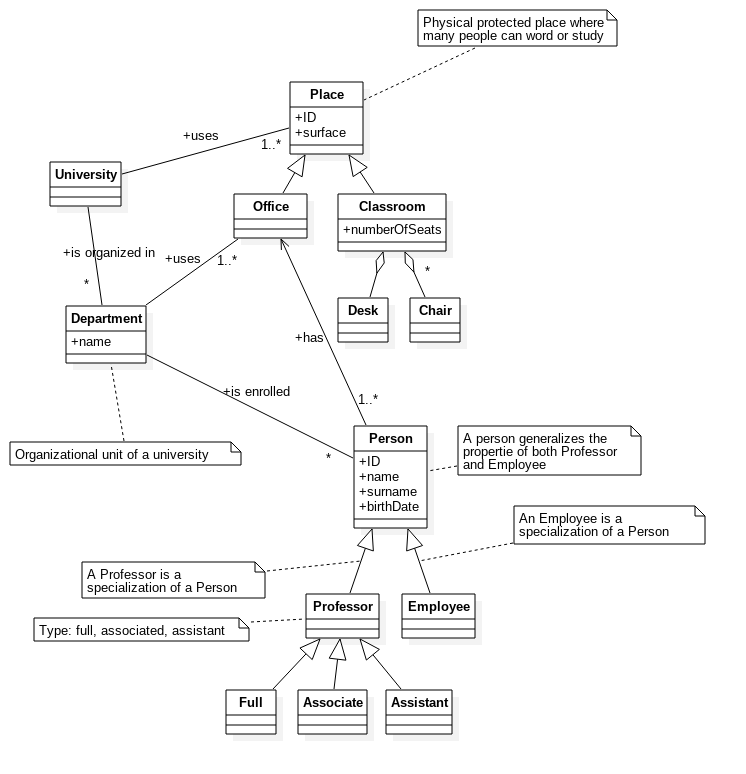
\includegraphics[scale=0.45]{exercises/classDiagram_university.png}
\caption{University - Class Diagram}
\end{figure}

\newpage
\section{Flights}
Draw a class diagram to define the glossary for management of flights and pilots.

An airline operates flights. Each airline has an ID. Each flight has an ID, a departure airport and an arrival airport: an airport has a unique identifier. Each flight has a pilot and a co-pilot, and it uses an aircraft of a certain type; a flight has also a departure time and an arrival time.

An airline owns a set of aircrafts of different types. An aircraft can be in a working state or it can be under repair, and in a particular moment an aircraft can be landed or airborne.

A company has a set of pilots: each pilot has an experience level: 1 is minimum, 3 is maximum.

A type of aircraft may need a particular number of pilots, with a different role (Ex. captain, co-pilot, navigator): there must be at least one captain and one co-pilot, and a captain must have a level 3.

\begin{sidewaysfigure}
\centering
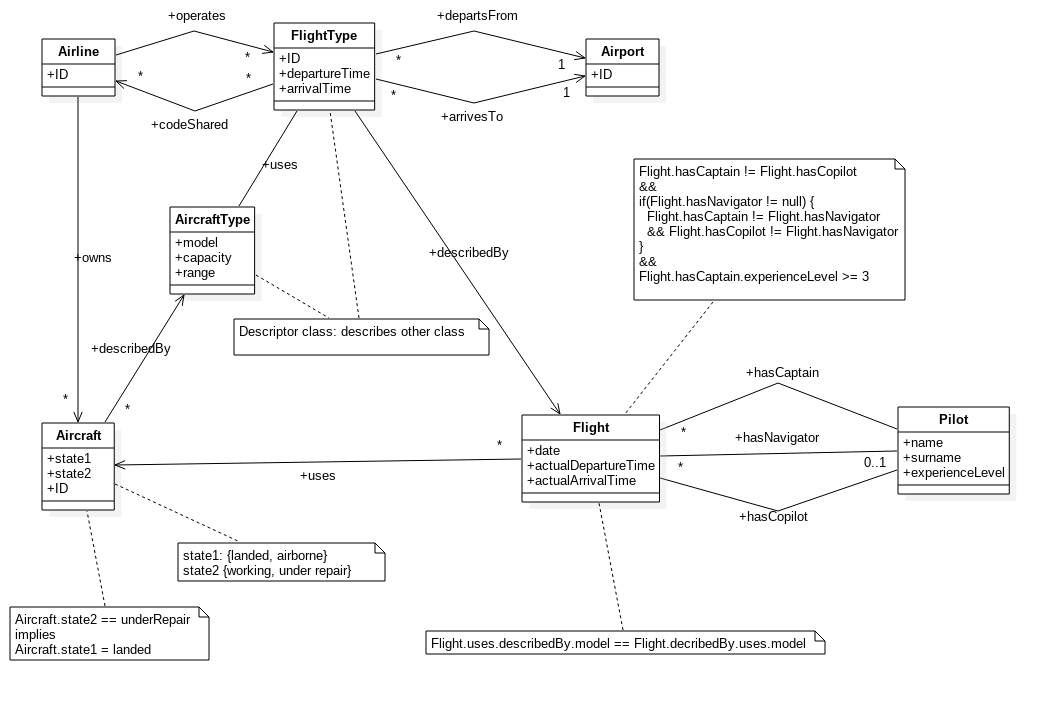
\includegraphics[scale=0.5]{exercises/classDiagram_flights.png}
\caption{Flights - Class Diagram}
\end{sidewaysfigure}
\chapter{Requirements engineering}
\emph{Requirements engineering} is about defining the product properties \emph{above starting development}. Without it, product properties may be unclear and testing phase is not feasible.

\textbf{Elicitation} consists of collecting information from the customer and producing an informal description, e.g.,\@ scratch or notes. This document is subjected to an analysis and formalization phase which produces the requirement document, a formal document which needs a final inspection in order to check its quality.

\begin{figure}[hbtp]
\centering
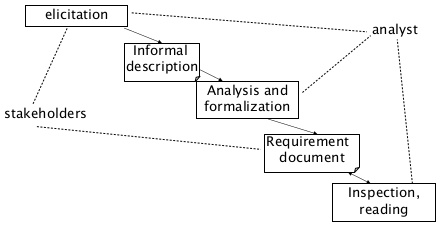
\includegraphics[scale=0.4]{images/re_phases.png}
\caption{Requirement engineering}
\end{figure}

A \textbf{requirement} is a description of a system or a service and its constraints. Requirements have different levels of abstraction and formality and they may be distinguished in functional and not functional.

Informal requirements often are not precisely stated. Ambiguous requirements may be interpreted in different ways by developers and users. In principle, requirements should be both complete and consistent.
\begin{itemize}
\item Complete: they should include descriptions of all facilities required;
\item Consistent: there should be no conflicts or contradictions in the descriptions of the system facilities.
\end{itemize}
In practice, it is impossible to produce a complete and consistent requirement document, also because there are no mathematical models or languages which can represent requirements.

\section{Defects}
\paragraph{Omission/Incompleteness}
Some information are not written. This defect is very difficult to find and fix.

\paragraph{Incorrect fact}
This defect is less difficult to find and fix. It may refer to a common knowledge.

\paragraph{Inconsistency/Ambiguity}
Some information are not strictly specified.

\paragraph{Extraneous information}
Overspecification: some information are not part of the requirement document.

\paragraph{Redundancy}
The same concept is repeated multiple times and possibly in slightly different ways, leading to ambiguity. Redundancy has to be avoided because, during the evolution of the document, it is possible to modify some concepts causing ambiguity.

\section{Techniques}
The requirement document is built using different techniques and it provides a \emph{structure}. The structure may change, order of parts is less important than precise description of parts.
\begin{enumerate}
\item Overall description;
\item Stakeholders;
\item Context diagram and interfaces;
\item Requirements
\begin{itemize}
\item Functional;
\item Non functional;
\item Domain;
\end{itemize}
\item Use case diagram;
\item Scenarios;
\item Glossary;
\item System design.
\end{enumerate}

\paragraph{Stakeholders}
A \emph{stakeholder} identifies a role or a person with an interest (stake) in the system to be built. Listing relevant stakeholders is essential to consider relevant points of view and therefore relevant requirements for the system.

\paragraph{Context diagram}
The \emph{context diagram} defines what is inside the system to be developed, what is outside and the interfaces between inside and outside. Outside entities interacting with the system are \textit{actors}. Stakeholders represent a subset of actors.

Context diagram and interfaces are essential to agree on what is the scope of the system.

\subparagraph{Interfaces}
Formal notations are an effective technique for interface specification.
Three types of interface may have to be defined:
\begin{itemize}
\item User interfaces, GUIs;
\item Procedural interfaces;
\item Data exchanged.
\end{itemize}

\paragraph{Numbering and type}
\begin{itemize}
\item Functional: general and informal description of services and behaviors provided by the system;
\item Non-functional: constraints on how functional requirements have to be implemented.
\end{itemize}

\subparagraph{Functional}
They can be inferred after the first reading of the informal description. Functional requirements are not all at the same level (i.e.,\@ complexity), in fact it is possible to introduce a hierarchy in requirements enumeration. Naming and numbering functional requirements is very useful because it helps their management (ready, released, paid) and their testing.

\subparagraph{Non-functional}
Non-functional requirements may be more critical than functional ones. If these are not met, the system is useless.
\begin{itemize}
\item Product requirements: requirements which specify that the delivered product must behave in a particular way (execution speed, reliability \dots);
\item Organizational requirements: requirements which are a consequence of organizational policies and procedures (process standard used, implementation requirements, \dots);
\item External requirements: requirements which arise from factors which are external to the system and its development process (interoperability requirements, legislative requirements, \dots).
\end{itemize}
Often, organizational and external requirements are taken for granted by the customer, therefore they are more difficult to extract.

ISO 9126 / ISO 25010 defines six properties of software systems associated to each function, not to the whole system.
\begin{itemize}
\item Functionality;
\item Reliability;
\item Usability\footnote{Waiting times < 0.1 sec are not perceived, while waiting > 1 sec are considered annoying.};
\item Efficiency;
\item Maintainability;
\item Portability.
\end{itemize}

Non-functional requirements must be \emph{measurable}, otherwise they are not testable, and therefore useless.

Conflicts between different non-functional requirements are common in complex systems. It is possible to rank the requirements in order to understand which are the most important.

\subparagraph{Domain requirements}
\emph{Domain requirements} are derived from the application domain and describe system characteristics and features reflecting the domain. They can be new functional requirements, constraints on existing requirements or define specific behaviors. If domain requirements are not satisfied, the system may be unworkable.

\textbf{Understandability}: requirements are expressed in the language of the application domain and they are often not understood by software engineers developing the system.

\textbf{Implicitness}: domain specialists understand them so well that they do not think of making the domain requirements explicit.

\paragraph{Glossary}
\emph{Glossary} is important to ``standardize'' terms. A class diagram can be used to refine glossary.

\paragraph{Scenarios}
A \emph{scenario} is a sequence of steps (events) that describe a typical interaction with the system. Each step should correspond to a function. In this way, it is possible to notice if a function is missing.

A scenario is also a \emph{test case}. Describing the interesting scenarios will help to perform 
coherent tests.

\paragraph{Use cases}
A \emph{use case} is a set of scenarios with common goal.

\paragraph{System design}
\emph{System design} identifies subsystems (software and not) composing the system.
\chapter{Black box testing}
\section{Int converter}
A function converts a sequence of chars in an integer number. The sequence can start with a `-' (negative number). If the sequence is shorter than 6 chars, it is filled with blanks (to the left side).

The integer number must be in the range minint = -32768 to maxint = 32767. The function signals an error if the sequence of chars is not allowed. The sequence of chars must be $\le 6$ chars.

\begin{itemize}
\item Define equivalence classes and related boundary conditions;
\item For each class, define at least one test case;
\item Define class Cartesian product. 
\end{itemize}
\texttt{int convert(string s);}

\subsection{Solution}
\paragraph{Criteria}
\begin{itemize}
\item Sign of the number: positive, negative;
\item Number length: $< 6$, $== 6$, $> 6$;
\item Well formed integer number: yes, no;
\item In range -32768, 32767: yes, no.
\end{itemize}
Actually, it is needed to combine different criteria. Table~\ref{tab:int_converter_first} shows some test cases which are not good enough, in fact some test cases, the ones highlighted, can belong to different classes and combinations have to be tested, too.

Table~\ref{tab:int_converter_second} shows how to perform criteria combinations. It is important to choose a ``good'' order for the criteria in order to prune as early as possible the number of combinations.

\begin{table}
\centering
\small
\begin{tabular}{|l|l|l|}
\hline
\textbf{Criterion} & \textbf{Valid} &\textbf{Invalid} \\
\hline
\multirow{4}{*}{Sign} & Positive & \\
&	{
	\begin{tabular}{l} % Positive
	T1(``1234''; 1234) \\
	\end{tabular}
	} & \\
\cline{2-2} % split positive and negative
& Negative & \\
&	{
	\begin{tabular}{l} % Negative
	T2(``-1234''; -1234) \\ 
	\end{tabular}
	} & \\
\hline % Sign end
\multirow{5}{*}{Length} & $< 6$ & $> 6$ \\
& 	{
	\begin{tabular}{l} % < 6
	T3(``12345''; 12345) \\
	\end{tabular}
	}
&	\multirow{4}{*}{ % > 6
	\begin{tabular}{l}
	\colorbox{yellow}{T6(``1234567''; error)} \\
	T7(``0004567''; error) \\
	\end{tabular}
	} \\
\cline{2-2} % split > 6 and == 6
& $== 6$ & \\
&	{
	\begin{tabular}{l} % = 6
	\colorbox{yellow}{T4(``123456''; error)} \\
	T5(``-12345''; -12345) \\
	\end{tabular}
	} & \\
\hline % Lenght end
\multirow{3}{*}{Well formed integer} & Y & N \\
&	{
	\begin{tabular}{l} % Yes
	T8(``234''; 234) \\
	T1 T2 T3 T5 \\
	\end{tabular}
	}
&	{
	\begin{tabular}{l} % No
	T9(``12ff99''; error) \\
	T10(``ff''; error) \\
	\end{tabular}
	} \\
\hline % Well formed end
\multirow{5}{*}{Range} & -32768, 32767 & > 32767 \\ 
&	\multirow{3}{*}{
	\begin{tabular}{l} % In range
	T1, T2, T3, T5, T8
	\end{tabular}
	}
&	{
	\begin{tabular}{l} % Not in range, greater
	T5 \\
	T11(``40000''; error)
	\end{tabular}
	} \\
\cline{3-3} % split out of range
& & < -32768 \\
& &	{
	\begin{tabular}{l}
	T12(``-40000''; error)
	\end{tabular}
	} \\
\hline
\end{tabular}
\caption{Int converter - Test cases}
\label{tab:int_converter_first}
\end{table}

\begin{table}
\centering
\small
\begin{tabular}{|l|l|l|l|l|}
\hline
\textbf{Sign} & \textbf{Length} & \textbf{Well formed} & \textbf{Range} & \textbf{Test cases} \\
\hline
\multirow{18}{*}{Positive} & \multirow{6}{*}{$< 6$} & \multirow{3}{*}{Yes} & -32768, 32767 & T1(``1234''; 1234) \\
\cline{4-5}
& & & > 32767 & T11(``40000''; error) \\
\cline{4-5}
& & & < -32768 & Unfeasible \\
\cline{3-5}
& & \multirow{3}{*}{No} & -32768, 32767 & \multirow{3}{*}{No sense} \\
\cline{4-4}
& & & > 32767 & \\
\cline{4-4}
& & & < -32768 & \\
\cline{2-5}
& \multirow{6}{*}{$> 6$} & \multirow{3}{*}{Yes} & -32768, 32767 & T7(``0004567''; error) \\
\cline{4-5}
& & & > 32767 & T6(``1234567''; error) \\
\cline{4-5}
& & & < -32768 & Unfeasible \\
\cline{3-5}
& & \multirow{3}{*}{No} & -32768, 32767 &  \multirow{3}{*}{No sense} \\
\cline{4-4}
& & & > 32767 & \\
\cline{4-4}
& & & < -32768 & \\
\cline{2-5}
& \multirow{6}{*}{$== 6$} & \multirow{3}{*}{Yes} & -32768, 32767 & T13(``012345''; 12345) \\
\cline{4-5}
& & & > 32767 & T14(``123456''; error) \\
\cline{4-5}
& & & < -32768 & Unfeasible \\
\cline{3-5}
& & \multirow{3}{*}{No} & -32768, 32767 & \multirow{3}{*}{No sense} \\
\cline{4-4}
& & & > 32767 & \\
\cline{4-4}
& & & < -32768 & \\
\cline{1-5}
\multirow{18}{*}{Negative} & \multirow{6}{*}{$< 6$} & \multirow{3}{*}{Yes} & -32768, 32767 & T2(``-1234''; -1234) \\
\cline{4-5}
& & & > 32767 & Unfeasible \\
\cline{4-5}
& & & < -32768 & Unfeasible \\
\cline{3-5}
& & \multirow{3}{*}{No} & -32768, 32767 & \multirow{3}{*}{No sense} \\
\cline{4-4}
& & & > 32767 & \\
\cline{4-4}
& & & < -32768 & \\
\cline{2-5}
& \multirow{6}{*}{$> 6$} & \multirow{3}{*}{Yes} & -32768, 32767 & T15(``-030000''; error) \\
\cline{4-5}
& & & > 32767 & Unfeasible \\
\cline{4-5}
& & & < -32768 & T16(``-400000''; error)  \\
\cline{3-5}
& & \multirow{3}{*}{No} & -32768, 32767 & \multirow{3}{*}{No sense} \\
\cline{4-4}
& & & > 32767 & \\
\cline{4-4}
& & & < -32768 & \\
\cline{2-5}
& \multirow{6}{*}{$== 6$} & \multirow{3}{*}{Yes} & -32768, 32767 & T5(``-12345''; -12345) \\
\cline{4-5}
& & & > 32767 & Unfeasible \\
\cline{4-5}
& & & < -32768 & T12(``-40000''; error) \\
\cline{3-5}
& & \multirow{3}{*}{No} & -32768, 32767 & \multirow{3}{*}{No sense} \\
\cline{4-4}
& & & > 32767 & \\
\cline{4-4}
& & & < -32768 & \\
\hline
\end{tabular}
\caption{Int converter - Criteria combinations}
\label{tab:int_converter_second}
\end{table}

\paragraph{Boundary conditions}
\begin{itemize}
\item Sign:
\begin{itemize}
\item T1boundary(``0''; 0)
\item T2boundary(``-0''; 0)
\end{itemize}
\item Well formed:
\begin{itemize}
\item T3boundary(``''; error)
\item T4boundary(``-''; error)
\end{itemize}
\item Range:
\begin{itemize}
\item T5boundary(``32767''; 32767)
\item T6boundary(``32768''; error)
\item T7boundary(``32766''; 32767)
\end{itemize}
\end{itemize}

\section{Calendar}
Consider a method that returns the number of days in a month, given the month and year.
\begin{verbatim}
public class MyGregorianCalendar {
  public static int getNumDaysInMonth(int month, int year) {
    ...
  }
  ...
}
\end{verbatim}
The month and the year are specified as integer. By convention, 1 represents January, 2 represents February and so on. The range of valid input for the year is 0 to \texttt{maxInt}. To determine leap years:
\begin{verbatim}
if year modulo 400 is 0 then leap
  else if year modulo 100 is 0 then no_leap
  else if year modulo 4 is 0 then leap
  else no_leap
\end{verbatim}

\paragraph{Equivalence classes}

\begin{itemize}
\item Month:
\begin{itemize}
\item Minint to 0;
\item 30 days \{4, 6, 9, 11\};
\item 31 days \{1, 3, 5, 7, 8, 10, 12\};
\item February \{2\};
\item 13 to Maxint.
\end{itemize}
\item Year:
\begin{itemize}
\item Minint to 0;
\item 1 to Maxint.
\end{itemize}
\end{itemize}
Test cases are shown in table~\ref{tab:calendar_test_cases}. Actually, since the number of month is limited, it is possible to explore all possible combination for each single month, not only for February. In this way, more test cases will be written and a better coverage is guaranteed, but this approach requires more time and effort in writing and running all test cases.

\paragraph{Boundary conditions}
In each partition, boundaries must be considered and test cases on boundary conditions have to be written.

\begin{table}
\centering
\small
\begin{tabular}{|l|l|c|l|}
\hline
\textbf{Month} & \textbf{Year} & \textbf{Leap condition} & \textbf{Test case} \\
\hline
\multirow{2}{*}{Minint to 0} & Minint to 0 & \multirow{2}{*}{-} & T1(-10, -10; error) \\
\cline{2-2} \cline{4-4}
& 1 to Maxint & & T2(-10, 10; error) \\
\hline
\multirow{2}{*}{\{4, 6, 9, 11\}} & Minint to 0 & \multirow{2}{*}{-} & T3(4, -10; error) \\
\cline{2-2} \cline{4-4}
& 1 to Maxint & & T4(6, 2000; 30) \\
\hline
\multirow{2}{*}{\{1, 3, 5, 7, 8, 10, 12\}} & Minint to 0 & \multirow{2}{*}{-} & T5(7, -10; error) \\
\cline{2-2} \cline{4-4}
& 1 to Maxint & & T6(7, 2000; 31) \\
\hline
\multirow{5}{*}{\{2\}} & Minint to 0 & - & T7(2, -10; error) \\
\cline{2-4}
& \multirow{4}{*}{1 to Maxint} & \multicolumn{1}{l|}{Year modulo 400} & T8(2, 2000; 29) \\
\cline{3-4}
& & \multicolumn{1}{l|}{Year modulo 100} & T9(2, 1900; 28) \\
\cline{3-4}
& & \multicolumn{1}{l|}{Year modulo 4} & T10(2, 1904; 29) \\
\cline{3-4}
& & \multicolumn{1}{l|}{Else} & T11(2, 1903; 28) \\
\hline
\multirow{2}{*}{13 to Maxint} & Minint to 0 & \multirow{2}{*}{-} & T12(14, -10; error) \\
\cline{2-2} \cline{4-4}
& 1 to Maxint & & T13(15, 2000; error) \\
\hline
\end{tabular}
\caption{Calendar - Test cases}
\label{tab:calendar_test_cases}
\end{table}

\section{Events}
A queue of events in a simulation system receives events. Each event ha s time tag. It is possible to extract events from the queue, the extraction must return the event with lower time tag. The queue discards events with negative or null time tag and accepts at most 100000 events. Events with the same tag must me merged, i.e.,\@ the second received is disregarded.
\begin{verbatim}
public class EventQueue {
  public void reset();
  public void push(int timeTag) throws InvalidTag, QueueOverflow;
  public int pop() throws EmptyQueue;
}
\end{verbatim}

\subsection{Push}
\begin{itemize}
\item Sign of the time tag ($\le 0$, $> 0$);
\item Number of events (0 to 100000, > 100000);
\item Repetitions of time tags (Yes, No).
\end{itemize}
Test cases are shown in table~\ref{tab:events_push}. Boundary for the time tag has to be considered, too.

\subsection{Pop}
These tests are quite similar to the push ones. Furthermore, they use the \texttt{push} function which has to be already tested, indeed. 

\begin{table}
\centering
\begin{tabular}{|l|l|l|l|}
\hline
\textbf{Time tag} & \textbf{\# Events} & Repetitions & \textbf{Test case} \\
\hline
\multirow{6}{*}{$\le 0$} & \multirow{4}{*}{0 to 100000} & \multirow{3}{*}{No} & T1 \\
\cline{4-4}
& & & TB1 \\
\cline{4-4}
& & & TB2 \\
\cline{3-4}
& & Yes & T2 \\
\cline{2-4}
& \multirow{2}{*}{> 100000} & No & T3 \\
\cline{3-4}
& & Yes & T4 \\
\hline
\multirow{6}{*}{$> 0$} & \multirow{2}{*}{0 to 100000} & No & T5 \\
\cline{3-4}
& & Yes & T6 \\
\cline{2-4}
& \multirow{4}{*}{> 100000} & \multirow{3}{*}{No} & T7 \\
& & & TB3 \\
& & & TB4 \\
\cline{3-4}
& & Yes & T8 \\
\hline
\end{tabular}
\caption{Events - Push test cases}
\label{tab:events_push}
\end{table}

\subsection{Test cases}
\begin{multicols}{2}
\paragraph{T1}
\begin{verbatim}
try {
  EventsQueue eq =
    new EventsQueue();
  eq.push(-10);
  eq.push(-12);
  eq.push(-14);
} catch() {
  InvalidTag
  success();
}
\end{verbatim}

\paragraph{T2}
\begin{verbatim}
try {
  EventsQueue eq =
    new EventsQueue();
  eq.push(-10);
  fail();
  eq.push(-10);
  eq.push(-10);
} catch() {
  InvalidTag
  success();
}
\end{verbatim}

\paragraph{T3}
\begin{verbatim}
try {
  EventsQueue eq =
    new EventsQueue();
  int i = 1;
  for(100010 times) {  
    eq.push(i--);
  }
  fail();
} catch() {
  InvalidTag or QueueOverflow
  success();
}
\end{verbatim}

\bigskip
\paragraph{T4}
\begin{verbatim}
try {
  EventsQueue eq =
    new EventsQueue();
  int i = 1;
  for(100010 times) {  
    eq.push(-10);
  }
  fail();
} catch() {
  InvalidTag or QueueOverflow
  success();
}
\end{verbatim}

\paragraph{T5}
\begin{verbatim}
try {
  EventsQueue eq =
    new EventsQueue();
  eq.push(10);
  eq.push(20);
  eq.push(30);
} catch() {
  fail();
}
eq.pop() == 10;
eq.pop() == 20;
eq.pop() == 30;
eq.pop() -> EmptyQueue;
\end{verbatim}

\paragraph{T6}
\begin{verbatim}
try {
  EventsQueue eq =
    new EventsQueue();
  eq.push(10);
  eq.push(10);
  eq.push(10);
} catch() {
  fail();
}
eq.pop() == 10;
eq.pop() -> EmptyQueue;
\end{verbatim}

\paragraph{T7}
\begin{verbatim}
try {
  EventsQueue eq =
    new EventsQueue();
  int i = 1;
  for(100010 times) {  
    eq.push(i++);
  }
  fail();
} catch() {
  QueueOverflow
  success();
}
\end{verbatim}

\paragraph{T8}
\begin{verbatim}
try {
  EventsQueue eq =
    new EventsQueue();
  for(100010 times) {  
    eq.push(10);
  }
} catch() {
  fail();
}
\end{verbatim}

\paragraph{TB1 - Empty and tag = 0}
\begin{verbatim}
try {
  EventsQueue eq =
    new EventsQueue();
  eq.push(0);
} catch() {
  InvalidTag
  success();
}
\end{verbatim}

\paragraph{TB2 - Tag = 0}
\begin{verbatim}
try {
  EventsQueue eq =
    new EventsQueue();
  eq.push(10);
  eq.push(0);
} catch() {
  InvalidTag
  success();
}
\end{verbatim}

\paragraph{TB3}
\begin{verbatim}
try {
  EventsQueue eq =
    new EventsQueue();
  int i = 1;
  for(100000 times) {  
    eq.push(i++);
  }
  pop() == 1;
} catch() {
  fail();
}
\end{verbatim}

\paragraph{TB4}
\begin{verbatim}
try {
  EventsQueue eq =
    new EventsQueue();
  int i = 1;
  for(100001 times) {  
    eq.push(i++);
  }
  fail();
  pop() == 1;
} catch() {
  success();
}
\end{verbatim}
\end{multicols}
\end{document}